\documentclass[12pt]{CSUNthesis}
%%%%%%%%%
\textheight=22cm
\def\T{\mathbb{T}}
\def\twotop#1#2{\genfrac{}{}{0pt}{}{#1}{#2}}
% % %
\def\R{\mathbb{R}}
% % % 

%%%%%%%%%
\usepackage{color}
\newcommand{\hl}[1]{\colorbox{lightgray}{#1}}
%\usepackage{tocloft}3
\usepackage{setspace}
\usepackage{amsmath}
\usepackage{amssymb}
\usepackage{graphicx}
%\usepackage{subfigure}
%\usepackage{epsfig}
\usepackage{epstopdf}
\usepackage{hyphenat}
\usepackage{setspace}
\usepackage{pdfsync}
\usepackage{tensor}
\usepackage{float}
\usepackage{subfig}
\restylefloat{table}

\setlength{\topmargin}{-0.25in}
\setlength{\textheight}{9.0in}
\setlength{\oddsidemargin}{0.5in} \setlength{\evensidemargin}{0.0in}
\setlength{\textwidth}{6.0in}

\newtheorem{example}{Example}
\newtheorem{theorem}{Theorem}
\newtheorem{proposition}{Proposition}
\newtheorem{corollary}[theorem]{Corollary}
\newtheorem{claim}[theorem]{Claim}
\newtheorem{definition}{Definition}
\newtheorem{remark}{Remark}[section]
\newtheorem{lemma}{Lemma}
\newtheorem{defn}{Definition}[section]

\newtheorem{rem}{Remark}[section]
\newenvironment{proof}[1][Proof]{\noindent\textbf{#1.} }{\newline \hspace*{\textwidth}\hspace*{-0,4cm} \rule{0.5em}{0.5em} \vspace{0,2cm}}

\renewcommand{\baselinestretch}{2}
\newcommand{\Rn}{$\mathbb{R}^n$}
\newcommand{\Rm}{$\mathbb{R}^m$}
\newcommand{\Rns}{$\mathbb{R}^n $ }
\newcommand{\Rnn}{$\mathbb{R}^{n+1}$}
\newcommand{\tb}{\textcolor{blue}}
\newcommand{\tr}{\textcolor{red}}
\newcommand{\D}{\mathrm{d}} % this defines a new command for making the d's in integrals look good
\newcommand{\limit}[3]{\underset{#1 \to #2}{\lim}  #3}  %this defines a command called limit with 3 slots
\newcommand{\manM}{$\mathcal{M}$}
\newcommand{\manMs}{$\mathcal{M} $ }
\newcommand{\Tref}{T_{\infty}}
\newcommand{\Cref}{C_{\infty}}
% Math mode friendly shortcuts
% % %
\def\T{\mathbb{T}}
\def\R{\mathbb{R}}
\def\Sbb{\mathbb{S}}
\def\e{\mathrm{e}}
\def\calF{\mathcal{F}}
\newcommand{\dydx}[2]{\frac{\partial{#1}}{\partial{#2}}}
\newcommand{\vecx}{\vec{x}}
\newcommand{\vecv}{\vec{v}}
\newcommand{\bulkv}{\vec{\bar{v}}} %bulk velocity


\newenvironment{Proof}[1][Proof]{\noindent\textbf{#1.} }{\newline \hspace*{\textwidth}\hspace*{-0,4cm} \rule{0.5em}{0.5em} \vspace{0,2cm}}
%%%%%%%%%

%% ADDITIONAL COMMANDS BEGIN


%%USE TIKPICTURE
\usepackage{tikz}
\usetikzlibrary{fit}
\usetikzlibrary{shapes}
\usetikzlibrary{arrows}
\usetikzlibrary{decorations.markings}
\usetikzlibrary{positioning}

\tikzset{mylabel/.style={font=\footnotesize}}
\tikzset{mymidlabel/.style={fill=white}}
%\tikzset{mymidlabel/.style={fill=white,font=\footnotesize}}

\definecolor{mydark}{RGB}{73,68,62}%{128,129,135}
\definecolor{mymedium}{RGB}{128,129,135}%{167,170,171}
\definecolor{mylight}{RGB}{226,226,226}
\definecolor{myyellow}{RGB}{251,214,0}
\definecolor{mydarkyellow}{RGB}{255,204,13}
%%%%%%%%%%%%%%%%%%%%%%%%%%%%%

\usepackage{lmodern}
\usepackage{mathtools}
\linespread{1.0}
\usepackage[font={small,it}]{caption}
\usepackage{tabularx}
\usepackage{sidecap}
\usepackage{colortbl,xcolor}

\usepackage{algorithm,algpseudocode}


% % % Additional Commands End

%%%%%%%%%

% Set the path to graphics.
\graphicspath{{images/}}

\submitted{August}{2015}

\author{Jeffrey Limbacher}

\title{Working title}

\committee {Alexander Alekseenko , Ph.D.}
		   {Ali Zakeri , Ph.D.}
           {Vladislav Panferov , Ph.D.}

\abstract{tbd}

%\copyrightyear{2015}

\acknowledgement{tbd}

\begin{document}
\doublespacing

%%%%%%%%%%%%%%%%%%%%%%%%%%%%%%%%%%%%%%%%%%%%%%%%%%%%%%%%%
%%%% CHAPTER ONE
%%%%%%%%%%%%%%%%%%%%%%%%%%%%%%%%%%%%%%%%%%%%%%%%%%%%%%%%%

\chapter{Introduction}
\label{Chap1}

%%%%%%%%%%%%%%%%%%%%%%%%%%%%%%%%%%%%%%%%%%%%%%%%%%%%%%%%%
%%%% CHAPTER TWO
%%%%%%%%%%%%%%%%%%%%%%%%%%%%%%%%%%%%%%%%%%%%%%%%%%%%%%%%%

\chapter{The Boltzmann Equation}
\label{Chap2}
	The kinematic theory of gases treats gases as composed of a large number of individual molecules that for large periods of time flow freely. As these particles move freely through space, they collide with each other. Collisions of these particles are what drive the evolution of the gas towards equilibrium. 
	
\section{Binary Collisions of Particles}
\label{sec:bincol}
	This section considers the properties of two particles on a collision path with each other as illustrated in Figure \ref{fig:binary_collision}. In all the work that follows, is is assumed that the molecules undergo elastic hard sphere collisions. 
\begin{figure}[h]
	\centering
	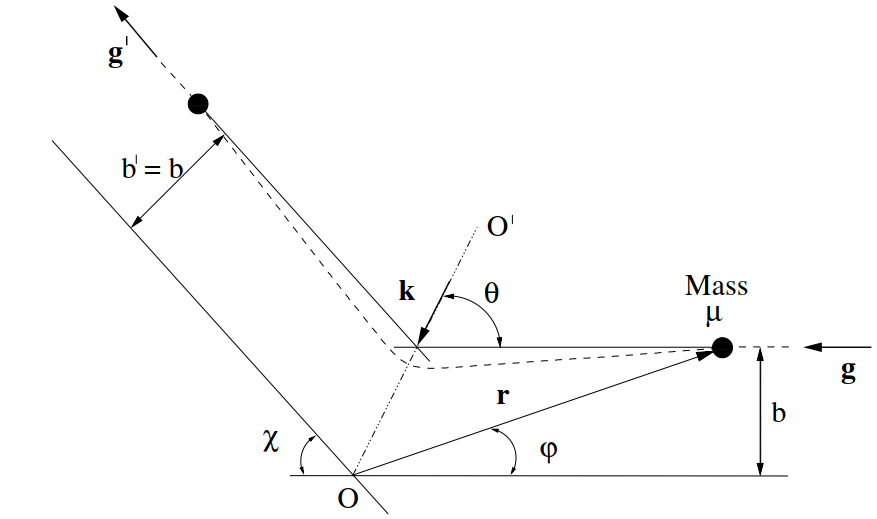
\includegraphics[scale=.5]{binary_collision}
	\caption{Kremer (2010, p. 27), Fig 1.6}
	\label{fig:binary_collision}
\end{figure}
	
	 Denote the pre- and post-collisional asymptotic velocities by $\vec{v}$, $\vec{v_1}$ and $\vec{v}'$, $\vec{v}_1'$ respectively. Define the relative pre- and post-collisional velocities, respectively, by 
\begin{equation*}
	\vec{g} = v_1 - v\, , \quad \vec{g}' = \vec{v}'-\vec{v}_1' \, .
\end{equation*}
$b$ denotes the offset of the centers of the molcules orthogonal to $\vec{g}$. $\varepsilon$ denotes the azimuthal angle between the two particles. 

By conservation of momentum, we have that 
\begin{equation}
\label{eq:consv_momentum}
m \vecv + m \vecv_1 = m\vecv' + m\vecv_1'\, .
\end{equation}
Equation \ref{eq:consv_momentum} yields $|g'| = |g|$. In addition, due to the hard sphere assumption, the collision is considered to be perfectly elastic, giving
\begin{equation}
\label{eq:consv_kin}
\frac{1}{2} m|\vecv| + \frac{1}{2} m|\vecv_1| = \frac{1}{2}m|\vecv'| + \frac{1}{2}m|\vecv_1'|
\end{equation}

The apsidal vector, $\vec{k}$ given by
\begin{equation*}
\vec{k} = \frac{\vec{g} - \vec{g}'}{|\vec{g} - \vec{g'}|}\, ,
\end{equation*}
bisects the angle between asymptotic relative velocities. Using this vector, we can write a relationship between the pre- and post-collisional velocities by
\begin{equation}
\label{eq:vel_relation}
\vec{v}_1' = \vec{v}_1 - \vec{k}(\vec{k} \cdot \vec{g})\, , \quad \vec{v}' = \vec{v} + \vec{k}(\vec{k} \cdot \vec{g})\, .
\end{equation}


\section{The Boltzmann Equation}

We consider a gas enclosed in a volume. A single molecule of this gas can be described with having position $\vec{x}$ and velocity $\vec{v}$ at a time $t$. For a particular time, we can describe a molecule as being within at a single point, $(\vec{x},\vec{v})$, in 6-dmensional space known as phase space. We define the distribution function of the gas as $f(t,\vec{x},\vec{v})d\vec{x}\,d\vec{v}$ gives the number of particles within the range of $\vec{x} + d\vec{x}$ with velocities $\vec{v} + d\vec{v}$. 

In 1872 Boltzmann \cite{Boltzmann1872} introduced the Boltzmann equation which describes the time evolution of the distribution $f$. In the absence of external forces and we ignore collisions of particles, then the Boltzmann equation takes the form
\begin{equation}
\label{eq:colless_boltzmann}
\dydx{}{t}f(t, \vecx, \vecv) + \vecv \cdot \nabla_x f(t, \vecx, \vecv) = 0\, .
\end{equation}
However, when the effects of collisions cannot be neglected, the right hand side must be modified to take this into account. In this case, the Boltzmann equation takes the form of
\begin{equation}
\label{eq:boltzmann}
\dydx{}{t}f(t, \vecx, \vecv) + \vecv \cdot \nabla_x f(t, \vecx, \vecv) = I[f](t,\vecx,\vecv)\, \\ 
\end{equation}
Where $I[f]$ is referred to as the collision operator. The explicit form of $I[f]$ depends on the properties of the gas. To describe it explicitly, we make several assumptions. First, the gas composed entirely of a single species of molecule. Second, we assume hard sphere collisions as described in section \ref{sec:bincol}. 

In order to explicitly write the collision operator, we must describe the collisions within the gas. Consider a particle with velocity $\vecv_1$ at point $\vecx$. This particle will collide with $f(t,\vecx, \vecv)d\vecv_1 g \Delta t b \, db \, d\varepsilon$ particles within the ranges of $\vecv_1$ and $\vecv_1 + d\vecv_1$. Integrating this by all all possible angles $(0 <= \varepsilon < 2 \pi)$, over all impact parameters, $(0 \leq b \leq b^*)$, and over all velocities, for all particles within the volume element $\vecx d\vecx$, we get that there are 
\begin{equation}
\label{eq:depletion}
dt \int_{\R^3} \int_0^{b^*} \int_0^{2\pi} f(t, \vecx, \vecv_1) f(t, \vecx, \vecv) b |g|\,  db \, d\varepsilon\, d\vecv_1 
\end{equation}
total collisions within the volume element that annihilate points with velocity $\vecv$. Likewise, there are collisions that create points with velocity $\vecv$. Using the results of the lasts section, points with velocity $\vecv'$ and $\vecv_1'$, impact parameter $b'=b$, and azimuthal angle $\varepsilon' = \pi + \varepsilon$ will result in particles with post-collisional velocity of $\vecv$ and $\vecv_1$. The number of such collisions is
\begin{equation}
\label{eq:restitution}
\begin{split}
&dt \int_{\R^3} \int_0^{b^*} \int_0^{2\pi} f(t, \vecx, \vecv_1') f(t, \vecx, \vecv') b' |g'|\,  db \, d\varepsilon'\, d\vecv_1 \,  \\
=&dt \int_{\R^3} \int_0^{b^*} \int_0^{2\pi} f(t, \vecx, \vecv_1') f(t, \vecx, \vecv') b |g|\,  db \, d\varepsilon\, d\vecv_1 \, .
\end{split}
\end{equation}

Subtracting (\ref{eq:depletion}) from (\ref{eq:restitution}) gives the net number of particles enter or leave the volume element $\vecv + d\vecv$; that is
\begin{equation}
\label{eq:explicit_I}
I[f](t, \vecx, \vecv) = \int_{\R^3} \int_{\R^3} (f_1' f' - f_1 f) |g|\, b\, db\, d\varepsilon\, d\vecv_1\, ,
\end{equation}
where,
\begin{equation*}
f_1' \equiv f(t, \vecx, \vecv_1')\quad f' \equiv f(t, \vecx, \vecv') \quad f_1 \equiv f(t, \vecx, \vecv_1 \quad f \equiv f(t, \vecx, \vecv)\, .
\end{equation*}
From here, we can substitute (\ref{eq:explicit_I}) into (\ref{eq:boltzmann}) to arrive to the explicit form of the Boltzmann equation,
\begin{equation}
\dydx{}{t}f(t, \vecx, \vecv) + \vecv \cdot \nabla_x f(t, \vecx, \vecv) = \int_{\R^3} \int_{\R^3} (f_1' f' - f_1 f) |g|\, b\, db\, d\varepsilon\, d\vecv_1\, .
\end{equation}
The Boltzmann equation is a non-linear integro-differential equation. The right hand side is a five dimensional integral that must be evaluated at each point in 6-dimensional space.

\section{Moments of the Distribution Function}

A gas is usually described by its macroscopic states. Kinetic theory defines these macroscopic properties in terms of distribution function $f(t,\vecx, \vecv)$. The first five moments of the gas are defined below.
\begin{align}
	n(t,\vec{x})&=\int_{\mathbb{R}^3}  f(t,\vec{x},\vec{v}) d\vec{v} &\text{- number density}  \label{eq:dens} \\
	\bar{v}_i(t,\vec{x})&=\frac{1}{n(t,\vec{x})} \int_{\mathbb{R}^3} m v_i f(t,\vec{x},\vec{v}) d\vec{v} &\text{- bulk velocity} \label{eq:bulk} \\
	T(t,\vec{x}) &= \frac{1}{3Rn(t,\vecx)}\int_{\mathbb{R}^3} m C^2 f(t,\vec{x},\vec{v}) d\vec{v} &\text{- temperature} \label{eq:temperature}
\end{align}
where $C_i=v_i-\bar{v}_i$, $C^2=C_1^2 + C_2^2 + C_3^2$, and $R$ is the specific gas constant. The number density $n(t, \vecx)$ denote the number of particles contained in our distribution. $\bulkv (t,\vecx)$ denotes that average velocity of particles within the gas. The temperature denotes the deviation form the average. 

An important property of the collision integral is that the first five moments are conservative (see \cite{Kremer2010}), that is
\begin{equation}
\label{eq:I_conservative}
\begin{split}
	\int_{\mathbb{R}^3}  I[f](t,\vec{x},\vec{v}) d\vec{v} = 0\, ,  \\
	\int_{\mathbb{R}^3} v_i I[f](t,\vec{x},\vec{v}) d\vec{v} = 0\, ,  \\
	\int_{\mathbb{R}^3} C^2 I[f](t,\vec{x},\vec{v}) d\vec{v} = 0 \, .
\end{split}
\end{equation}

\section{The Maxwellian Distribution}

If the gas is free from external influence, then the gas will approach an equilibrium. In this equilibrium, the gas distribution takes a specific shape known as the Maxwellian distribution given below.
\begin{equation}
\label{eq:maxwellian}
f_M(\vec{v},n,\vec{\bar{v}},T) = \frac{1}{\sqrt{2 \pi R T}^3} \exp\left( -\frac{ |\vec{v} - \vec{\bar{v}}|^2}{2RT} \right)
\end{equation} 
	
Note that the exact shape of the Maxwellian distribution depends on the macroscopic moments of the gas distribution, $n$, $\vec{\bar{v}}$, and $T$ given by equations \ref{eq:dens}, \ref{eq:bulk}, \ref{eq:temperature} respectively. This is illustrated in Figure \ref{fig:1d_maxwellian}. The distribution is centered around $\bulkv$. The temperature, $T$, controls the width of the distribution. $n$ determines the area under the curve.
\begin{figure}[h]
\centering
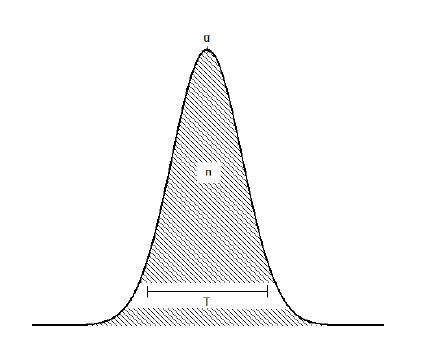
\includegraphics[scale=.5]{1D_Maxwellian}
\caption{Stolen picture need better caption}
\label{fig:1d_maxwellian}
\end{figure}

When the gas is in equilibrium, the difference between the number of particles that enter and leave a particular phase volume vanishes. In other words, 
\begin{equation*}
I[f_M](t,\vecx,\vecv) = \int_{\R^3} \int_{\R^3} (f_{M1}'f_M' - f_{M1} f_M)  g\, b\, db\, d\varepsilon\, d\vecv_1\ = 0
\end{equation*}

\section{Dimensionless Reduction}

Gas dynamic constants can vary greatly in scale. This can cause an accumulation of round-off error using floating point arithmetic when performing a large number of computations. In order to reduce the error that can be introduced by the varying scales, a dimensionless reduction is performed on the constants and equations. The dimensionless reduction aims to reduce the scale of all the variables to roughly of order one to minimize the round-off error. Note that the dimensionless reduction process can never eliminate round-off error since it is inherit to floating point arithmetic. The techniques used for dimensionless reduction vary from problem to problem. This thesis adopts the convention borrowed from Chapter 3 of [][][][].

Let $\hat{t}$, $\hat{x}$, and $\hat{v}$ denote the conventional dimensional variables. In general, all quantities bearing $\hat{\cdot}$ will represent dimensional quantities, i.e. whose numbers have units understood to have physical meaning (e.g.. seconds, meters, meters per second). For example, $\hat{f}(\hat{t},\hat{x},\hat{v})$ will represent the molecular number density distribution function.

We assume some time scale $\mathbb{T}$, reference temperature $\Tref$, and some length scale $L$, which are selected with a particular application in mind. We define $\Cref = \sqrt{2R\Tref}$. In addition, we define
\begin{equation}
\label{eq:new_dimless}
t=\frac{\hat{t}}{\T},
\quad x_{i}=\frac{\hat{x}}{L},
\quad v=\frac{\hat{v}}{C_{\infty}}, 
\quad \mbox{or}
\quad \hat{t}=t\T,
\quad \hat{x}=x L,
\quad \hat{v}=vC_{\infty}\, .
\end{equation}
The dimensionless density is
\begin{equation}
f(t,x,v) = \frac{L^3 \Cref^3}{N} \hat{f}(t\mathbb{T},xL, v\Cref) = \hat{f}(\hat{t},\hat{x},\hat{v})\, ,
\end{equation}
where $N$ is total number of molecules in the gas volume $L^3$. 

With these definitions, then the relationship between the dimensionless macroparameters and the dimensional pacroparameters are now as follows. We define
\begin{equation}
\begin{split}
\label{eq:dimless_macro}
n(t,x)&:=\int_{\R^3} f(t,x,v)  dv\, ,  \\
n(t,x)\bar{u}(t,x)&:=\int_{\R^3} vf(t,x,v) dv\,  ,  \\
n(t,x)T(t,x)&:=\frac{2}{3} \int_{\R^3} (v - \bar{u})^2 f(t,x,v) dv\, , 
\end{split}
\end{equation}

From the above definitions, we get the relationships of the dimensionless and dimensional macroparameters. First note that in the discussion of follows, we have $d\hat{v} = C_{\infty}^3 dv$. Then,
\begin{equation}
\begin{split}
n(t,x) &= \int_{\R^3} f(t,x,v)  dv\, \\
&= \int_{\R^3} \frac{L^3 \Cref^3}{N} \hat{f}(\hat{t},\hat{x},\hat{v})\frac{d\hat{v}}{\Cref^3} \\
&= \frac{L^3}{N}  \int_{\R^3}  \hat{f}(\hat{t},\hat{x},\hat{v}) d\hat{v}\\
&= \frac{L^3}{N} \hat{n}(t\T,xL)\, .
\end{split}
\end{equation}
In addition,
\begin{equation}
\begin{split}
n(t,x) \bar{u}_i(t,x) &= \int_{\R^3} v_j f(t,x,v)  dv\, \\
&= \int_{\R^3} \frac{L^3 \Cref^3}{N} \frac{\hat{v}_j}{\Cref} \hat{f}(\hat{t},\hat{x},\hat{v})\frac{d\hat{v}}{\Cref^3} \\
&= \frac{L^3}{\Cref N}  \int_{\R^3} \hat{v}_j  \hat{f}(\hat{t},\hat{x},\hat{v}) d\hat{v}\\
&= \frac{L^3}{\Cref N} \hat{n}(t,x,v) \hat{\bar{u}}(\hat{t},\hat{x}) d\hat{v} \\
&= \frac{\hat{\bar{u}}_j(t,x)}{\Cref}n(t,x)\, ,
\end{split}
\end{equation}
and
\begin{equation}
\begin{split}
n(t,x)T(t,x) &= \frac{2}{3} \int_{\R^3}(v-\bar{u})^2 f(t,x,v)dv \\
&= \frac{2}{3} \int_{\R^3} \frac{L^3 \Cref^3}{N} \left( \left( \frac{\hat{v}}{\Cref} \right)^2 - \left( \frac{\hat{\bar{u}}}{\Cref} \right)^2 \right)\hat{f}(\hat{t},\hat{x},\hat{v} \frac{d\hat{v}}{\Cref^3} \\
&= \frac{2L^3}{3 \Cref^2 N} \int_{\R^3} (\hat{v} - \hat{\bar{u}})^2\hat{f}(\hat{t},\hat{x},\hat{v}) d\hat{v} \\
&= \frac{L^3}{\Tref N }\hat{n}(\hat{t},\hat{x}) T(\hat{t},\hat{x}) \\ 
&= n(t,x) \frac{\hat{T}(\hat{t},\hat{x})}{\Tref} \, .\\
\end{split}
\end{equation}
To summarize the above results,
\begin{equation}
\begin{split}
n(t,x)&=\frac{L^3 }{N} \hat{n}(\hat{t},\hat{x})\, , \nonumber  \\
\bar{u}(t,x)&=\frac{\bar{\hat{u}}(\hat{t},\hat{x})}{\Cref}\, , \nonumber \\ 
T(t,x) &= \frac{\hat{T}(\hat{t},\hat{x})}{T_{\infty}} \, . \\
\end{split}
\end{equation}

Next, the Maxwellian distribution with density $\hat{n}(\hat{t},\hat{x})$, average velocity 
$\hat{\bar{u}}_{j}(\hat{t},\hat{x})$ and temperature $\hat{T}(\hat{t},\hat{x})$ translates 
into the dimensionless Maxwellian distribution as follows:
\begin{equation}
\begin{split}
\hat{f}_{M}(\hat{t},\hat{x},\hat{u}) &= \hat{n}(2\pi R\hat{T})^{-3/2} \exp \left(- \frac{(\hat{u}-\hat{\bar{u}})^2}{2R\hat{T}}\right) \\
&= \hat{n}(2 \pi R T)^{-3/2}(\Tref / \hat{T}) ^{3/2} \exp \left(- \frac{(\hat{u}-\hat{\bar{u}})^2}{2R \Tref}\frac{\Tref}{\hat{T}}\right)\\
&= \hat{n}\pi^{-3/2} \Cref^{-3} (1/T) ^{3/2} \exp \left(- \frac{(\hat{u}-\hat{\bar{u}})^2}{T}\right)\\
&= n \frac{N}{L^3 \Cref^3} (\pi T)^{-3/2} \exp \left(- \frac{(\hat{u}-\hat{\bar{u}})^2}{T}\right)\\
&=\frac{N}{L^3 C^3_{\infty}} f_{M}(t,x,u)\, ,
\end{split}
\end{equation}
where 
\begin{equation}
f_{M}(t,x,u) :=  \frac{n}{(\pi T)^{3/2}} \exp\Bigl(-\frac{(u-\bar{u})^2}{T} \Bigr )\, . 
\end{equation}

%%%%%%%%%%%%%%%%%%%%%%%%%%%%%%%%%%%%%%%%%%%%%%%%%%%%%%%%%
%%%% CHAPTER THREE
%%%%%%%%%%%%%%%%%%%%%%%%%%%%%%%%%%%%%%%%%%%%%%%%%%%%%%%%%

\chapter{Discontinuous Galerkin Discretization in the Velocity Variable}

Discontinuous Galerkin methods is a method of discretizing equations. The following section describes the DG formulation found in~\cite{AlekseenkoJosyula2012},~\cite{AlekseenkoNguyenWood2015}.

\section{DG Discretization in Velocity Space}
We denote the points in the velocity space as $\vec{v} = (u,v,w)$. The velocity space is reduced to a rectangular parallelpiped $K=[u_L, u_R] \times [v_L,v_R] \times [w_L,w_R]$. It is assumed that outside the parallelpiped the contribution of the function to the first few moments is negligible. Depending on the parallelpiped, this will not result in large errors in terms of conservation of density and temperature. 

We partition $K$ into $N$ smaller rectangular parallelpipeds $K_j = [u_L^j, u_R^j] \times [v_L^j, v_R^j] \times [w_L^j, w_R^j]$. Each $K_j$ will contain a set of basis function, $\phi_j^i$, $i=1,\dots, s$ as described. We introduce nodes of Gauss quadratures of order $s_u$, $s_v$, and $s_w$ on each of the intervals $[u_L^j,u_R^j]$, $[v_L^j,v_R^j]$, and $[w_L^j,w_R^j]$. The nodes are denoted as
$\kappa^{u}_{p;j}$, $\dots$, $p=1,s_{u}$,
$\kappa^{v}_{q;j}$, $\dots$, $q=1,s_{v}$, and 
$\kappa^{w}_{r;j}$, $\dots$, $r=1,s_{w}$. From the nodes, the one-dimensional Lagrange basis functions are defined:
\begin{equation}
\label{eq:01}
\phi^{u}_{l;j}(u)=\prod_{{p=1,s_{u}} \atop {p\neq l}} \frac{\kappa^{u}_{p;j}-u}{\kappa^{u}_{p;j}-\kappa^{u}_{l;j}}\, ,\quad 
\phi^{v}_{m;j}(v)=\prod_{{q=1,s_{v}} \atop {q\neq m}} \frac{\kappa^{v}_{q;j}-v}{\kappa^{v}_{q;j}-\kappa^{v}_{m;j}}\, ,\quad 
\phi^{w}_{n;j}(w)=\prod_{{r=1,s_{w}} \atop {r\neq n}} \frac{\kappa^{w}_{r;j}-w}{\kappa^{w}_{r;j}-\kappa^{w}_{n;j}}\, .
\end{equation}
The three-dimensional basis function is defined as
\begin{equation}
\label{eq:01a}
\phi_{i;j}(\vec{v})=\phi^{u}_{l;j}(u)\phi^{v}_{m;j}(v)
\phi^{w}_{n;j}(w)
\end{equation} 
where $l=1, \dots , s_u$, 
$m=1,\dots ,s_v$, 
$n=1,\dots ,s_w$ and $i$ 
is the index that runs through all possible combinations of $l$, $n$, and $m$, and is computed as $i=((l-1)s_v)+(m-1)s_w)+n$.  
A useful property of the basis functions (\ref{eq:01a}) is that they vanish on all nodes except one. In addition, the quadrature nodes used are exact on polynomials of degree at most $2s_u-1$, $2s_v-1$, and $2s_w-1$. In addition, the following lemma holds,
\begin{lemma} (see also \cite{AlekseenkoJosyula2012a, HesthavenWarburtoin2007})
The following identities hold for basis functions $\phi_{i;j}(\vec{v})$:
\begin{equation}
\label{eq:lemma2.1} 
\int_{K_{j}} \phi_{p;j}(\vec{v})\phi_{q;j}(\vec{v})\, d\vec{v} = \frac{\omega_{p}\Delta\vec{v}^{j}}{8}\delta_{pq}
\qquad\mbox{and} \qquad
\int_{K_{j}} \vec{v}\phi_{p;j}(\vec{v})\phi_{q;j}(\vec{v})\, d\vec{v} 
= \frac{\omega_{p}\Delta\vec{v}^{j}}{8}\vec{v}_{p;j}\delta_{pq},
\end{equation}
where indices $l$, $n$, and $m$ of one dimensional basis functions correspond to 
the three-dimensional basis functions 
$\phi_{p;j}(\vec{v})=
\phi^{u}_{l;j}(u)\phi^{v}_{m;j}(v)\phi^{w}_{n;j}(w)$, 
and the vector $\vec{v}_{p;j}=(\kappa^{u}_{l;j},\kappa^{v}_{m;j},\kappa^{w}_{n;j})$. 
\end{lemma}
\section{Nodal-DG Velocity Discretization of the Boltzmann Equation}
We assume that on each $K_j$, the solution to the Boltzmann equation is sought of the form 
\begin{equation}
\label{eq:3.4}
f(t,\vec{x},\vec{v})|_{K_{j}} = \sum_{i=1,s} f_{i;j}(t,\vec{x})\phi_{i;j}(\vec{v})\, .
\end{equation}
We substitute equation \ref{eq:3.4} into $\ref{eq:boltzmann}$, multiply the result by test basis function, integrate over $K_j$, and apply identity (\ref{eq:lemma2.1}) to arrive to
\begin{equation}
\label{discveloblzm}
\partial_{t} f_{i;j}(t,\vec{x}) + \vec{v}_{i;j}\cdot \nabla_{x} f_{i;j}(t,\vec{x}) =
\frac{8}{\omega_{i}\Delta\vec{v}^{j}}I_{\phi_{i;j}}\, ,
\end{equation}
where $I_{\phi_{i;j}}$ is the projection of the collision operator 
on the basis function $\phi_{i;j}(\vec{v})$:
\begin{equation}
\label{eq:projcoll}
I_{\phi_{i;j}} = \int_{K_{j}}\phi_{i;j}(\vec{v}) I[f](t,\vec{x},\vec{v})\, d\vec{v}\, .
\end{equation} 

\section{Reformulation of the Galerkin Projection of the Collision Operator}
\label{sec:reform_galerkin}
Similarly to \cite{AlekseenkoJosyula2012,AlekseenkoJosyula2012a,Majorana2011}, we rewrite the 
DG projection of the collision operator $I_{\phi_{i;j}}$ in the form of a bilinear integral operator 
with a time-independent kernel. The principles of kinetic theory suggest that changes to $f(t,\vecx, \vecv)$ with respect to $\vecx$ at the distance of a few $b^*$ are negligible, see e.g., \cite{Struchtrup2005}. Specifically, using the well-known identities (see, e.g.,  \cite{Kogan1969}, Section 2.4), and applying the first principles assumption, we have 
\begin{align}
\label{eq:transfer_eq}
I_{\phi_{i;j}}&= \int_{\R^3}\int_{\R^3} f(t,\vec{x},\vec{v}) f(t,\vec{x},\vec{v}_{1})
\int_{\Sbb^2}(\phi_{i;j}(\vec{v}')-\phi_{i;j}(\vec{v})) b_{\alpha}(\theta) |g|^\alpha \, d\sigma\,
 d\vec{v}_{1}\, d\vec{v} \nonumber \\
{} & = \int_{\R^3}\int_{\R^3} f(t,\vec{x},\vec{v}) f(t,\vec{x},\vec{v}_{1})
 A(\vec{v},\vec{v}_{1};\phi_{i;j})   d\vec{v}_{1}\, d\vec{v}\, ,
\end{align}
where  
\begin{align}
\label{eq:A_definition}
A(\vec{v},\vec{v}_{1};\phi_{i;j})= |g|^\alpha \int_{\Sbb^2} (\phi_{i;j}(\vec{v}')
- \phi_{i;j}(\vec{v})) b_{\alpha}(\theta) \, d\sigma\, .
\end{align}
The kernel $A(\vec{v},\vec{v}_{1};\phi_{i;j})$ is independent of time and can be pre-computed. 
In \cite{AlekseenkoJosyula2012a} properties of a kernel closely related to $A(\vec{v},\vec{v}_{1};\phi_{i;j})$ 
are considered.
In particular, due to the local support of $\phi_{i;j}(\vec{v})$, it is anticipated that 
kernel  $A(\vec{v},\vec{v}_{1};\phi_{i;j})$ will have only $O(M^{5})$ non-zero components for each $\phi_{i;j}(\vec{v})$, 
where $M$ is the number of discrete velocity points in each velocity dimension. As a result, evaluation of  
(\ref{eq:transfer_eq}) will require $O(M^{8})$ operations for each spatial point. This number of evaluations 
is very high. However, as we will show later, it can be reduced to $O(M^6)$ operations using symmetries of
$A(\vec{v},\vec{v}_{1};\phi_{i;j})$, the convolution form of (\ref{eq:transfer_eq}) and the Fourier 
transform. 

We remark that in many numerical re-formulations of the Boltzmann equation, the collision 
operator is separated into the gain and loss terms.
This separation can be performed in (\ref{eq:transfer_eq}),
\begin{align}
\label{eq:I_split}
I_{\phi_{i;j}}&= \int_{\R^3}\int_{\R^3} f(t,\vec{x},\vec{v}) f(t,\vec{x},\vec{v}_{1})
\int_{\Sbb^2}(\phi_{i;j}(\vec{v}')-\phi_{i;j}(\vec{v})) b_{\alpha}(\theta) |g|^\alpha \, d\sigma\,
 d\vec{v}_{1}\, d\vec{v} \nonumber \\
&= \int_{\R^3}\int_{\R^3} f(t,\vec{x},\vec{v}) f(t,\vec{x},\vec{v}_{1}) (\int_{\Sbb^2}\phi_{i;j}(\vec{v}')b_{\alpha}(\theta) |g|^\alpha d\sigma\, - |g|^\alpha\int_{\Sbb^2}\phi_{i;j}(\vec{v})b_{\alpha}(\theta)  d\sigma\,)  d\vec{v}_{1}\, d\vec{v} \nonumber \\
&= \int_{\R^3}\int_{\R^3} f(t,\vec{x},\vec{v}) f(t,\vec{x},\vec{v}_{1}) (A^+(\vecv,\vecv_1;\phi_{i;j}) - |g|^\alpha \sigma_T)  d\vec{v}_{1}\, d\vec{v}
\end{align}
where
\begin{equation}
\label{eq:A_split}
A^+(\vecv,\vecv_1;\phi_{i;j}) = \int_{\Sbb^2}\phi_{i;j}(\vec{v}')b_{\alpha}(\theta) |g|^\alpha d\sigma\, , \quad \sigma_T = \int_{\Sbb^2}\phi_{i;j}(\vec{v})b_{\alpha}(\theta)  d\sigma\, .
\end{equation}
$A^+(\vecv,\vecv_1;\phi_{i;j})$ has similar properties to that of $A(\vecv,\vecv_1;\phi_{i;j})$, but
$A^+(\vecv,\vecv_1;\phi_{i;j})$ has certain properties that are better than that of $A(\vecv,\vecv_1;\phi_{i;j})$ for a Fourier transform. 
$A(\vecv,\vecv_1;\phi_{i;j})$ is grows linearly to infinity in some direction whereas $A^+(\vecv,\vecv_1;\phi_{i;j})$ does not. It can then be argued that $A^+(\vecv,\vecv_1;\phi_{i;j})$ is better suited for a Fourier transform than $A(\vecv,\vecv_1;\phi_{i;j})$. The algorithms in this paper also have straightforward extensions to the the split formulation of (\ref{eq:transfer_eq}). However, in practice, the split formulation of (\ref{eq:transfer_eq}) had significant errors in conservation.

\section{Properties of the Kernel $A(\vecv,\vecv_1;\phi_{i;j})$}
\label{sec:props_of_a}
\begin{lemma}
\label{lem1} 
Let operator $A(\vec{v},\vec{v}_{1};\phi_{i;j})$ be defined by (\ref{eq:A_definition}). Then $\forall\xi\in \R^3$
\begin{equation*}
A(\vec{v}+\vec{\xi},\vec{v}_{1}+\vec{\xi};\phi_{i;j}(\vec{v}-\vec{\xi}))=
A(\vec{v},\vec{v}_{1};\phi_{i;j}) \, .
\end{equation*}
\end{lemma}

\proof
Consider $A(\vec{v}+\vec{\xi},\vec{v}_{1}+\vec{\xi};\phi_{i;j}(\vec{v}-\vec{\xi}))$. We clarify that these notations mean that
particle velocities $\vec{v}$ and $\vec{v}_{1}$ in (\ref{eq:A_definition}) are replaced with $\vec{v}+\vec{\xi}$ and $\vec{v}_{1}+\vec{\xi}$
correspondingly and that basis function $\phi_{i;j}(\vec{v})$ is replaced with a ``shifted'' function 
$\phi_{i;j}(\vec{v}-\vec{\xi})$. We notice that the relative speed of the molecules with velocities $\vec{v}+\vec{\xi}$ 
and $\vec{v}_{1}+\vec{\xi}$ is still $\vec{g}=\vec{v}+\vec{\xi}-(\vec{v}_{1}+\vec{\xi}_{1})=\vec{v}-\vec{v}_{1}$. 
The post-collision velocities for the pair of particles will be $\vec{v}'+\vec{\xi}$ and $\vec{v}'_{1}+\vec{\xi}$, where $\vec{v}'$ and $\vec{v}'_{1}$ are given by (\ref{eq:vel_relation}). We notice, in particular, that choices of $\theta$ and $\varepsilon$ in 
(\ref{eq:vel_relation}) are not affected by $\vec{\xi}$. The rest of the statement follows by a direct substitution:
\begin{align*}
A(\vec{v}&+\vec{\xi},\vec{v}_{1}+\vec{\xi};\phi_{i;j}(\vec{v}-\vec{\xi})) = |g|^{\alpha} \int_{\Sbb^2} \phi_{i;j}((\vec{v}'+\vec{\xi})-\vec{\xi}) b_{\alpha}(\theta)\, d\sigma\,= |g|^{\alpha} \int_{\Sbb^2} \phi_{i;j}(\vec{v}') b_{\alpha}(\theta)\, d\sigma \\
&  = A(\vec{v},\vec{v}_{1};\phi_{i;j})\, . 
\end{align*}
\endproof
We remark that Lemma~{\ref{lem1}} holds for all potentials of molecular 
interaction used in rarefied gas dynamics. This property was used in 
\cite{AlekseenkoJosyula2012a} to reduce the storage requirement 
on uniform partitions. 

\section{Rewriting the Collision Operator in the Form of a Convolution (Mostly Copy and Pasted from the Paper, needs rewrite?)}
It was shown in~\cite{AlekseenkoNguyenWood2015} that the Galerkin projection of the collision operator can be reformulated in terms of a convolution. This work is recalled in this section. 
We select a partition cell $K_c$ and designate this cell as a generating cell. 
Similarly, the basis functions $\phi_{i;c}(\vec{v})$ on $K_c$ are designated as the generating basis functions. 
Basis functions $\phi_{i;j}(\vec{v})$ on other cells can be obtained using a shift in the velocity variable, namely $\phi_{i;j} (\vec{v})=\phi_{i;c} (\vec{v}+\vec{\xi_{j}})$ where $ \vec{\xi}_{j} \in \mathbb{R}^3$ is the vector that connects the center of $K_j$ to the center of $K_c$.

According to  Lemma~{\ref{lem1}}, operator $A(\vec{v},\vec{v}_1,\phi_{i;j})$ is invariant with respect to translations. Therefore
\begin{align}
\label{eq3.1}
I_{\phi_{i;j}} &= \int_{\R^3}\int_{\R^3} f(t,\vec{x},\vec{v})f(t,\vec{x},\vec{v}_{1})A(\vec{v}+\vec{\xi_{j}},\vec{v}_1+\vec{\xi_{j}}; \phi_{i;j}(\vec{u} - \vec{\xi_{j}})) \, d\vec{v}_{1} d\vec{v} \notag\\
 &= \int_{\R^3}\int_{\R^3} f(t,\vec{x},\vec{v})f(t,\vec{x},\vec{v}_{1})A(\vec{v}+\vec{\xi^{j}},\vec{v}_{1}+\vec{\xi_{j}}; \phi_{i;c}(\vec{u})) \, d\vec{v} d\vec{v_{1}} \, .
\end{align}
Performing the substitutions $\vec{\hat{v}} = \vec{v}+\vec{\xi_{j}} $ and $ \vec{\hat{v}}_1 = \vec{v}_{1}+\vec{\xi_{j}}$ in (\ref{eq3.1}), we have
\begin{equation*}
I_{\phi_{i;j}} = \int_{\R^3}\int_{\R^3} f(t,\vec{x},\vec{\hat{v}}-\vec{\xi_{j}}) f(t,\vec{x},\vec{\hat{v}}_1-\vec{\xi_{j}}) A(\vec{\hat{v}},\vec{\hat{v}}_{1};\phi_{i;c}(\vec{u})) \, d\vec{\hat{v}} d\vec{\hat{v}}_1 \, .
\end{equation*}
We then introduce a bilinear convolution operator, $i=1,\ldots,s$
\begin{equation}
\label{eq:continuous_convolution}
I_i(\vec{\xi}) = \int_{\R^3}\int_{\R^3} f(t,\vec{x},\vec{v}-\vec{\xi})f(t,\vec{x},\vec{v}_{1}-\vec{\xi})A(\vec{v},\vec{v}_{1}; \phi_{i;c}) \, d\vec{v} d\vec{v}_{1} \, ,
\end{equation}
and notice that $I_{\phi_{i;j}}$ can be obtained from (\ref{eq:continuous_convolution}) as
$I_{\phi_{i;j}}=I_i(\vec{\xi}_j)$. In the following, we will refer to (\ref{eq:continuous_convolution}) 
as the convolution form of the Galerkin projection of the collision integral.

\section{Discretization of the Collision Integral (COpy and pasted again)}
In order to calculate (\ref{eq:continuous_convolution}), we replace the three-dimensional integrals with the Gauss quadratures associated with then nodal-DG discretization, (\ref{eq:01a}). 
As is discussed above, we are only interested in 
computing convolution (\ref{eq:continuous_convolution}) at vectors 
$\vec{\xi}=\vec{\xi}_{j}$ that connect centers of the velocity cells $K_j$ to the 
center of the velocity cell $K_c$, the support of $\phi_{i;c}(\vec{v})$. Since the 
same nodal points are used on all velocity cells, shifts $\vec{\xi}_{j}$ 
translate nodal points in one cell to nodal points 
in another cell. As a result, the quadrature sums to evaluate convolution (\ref{eq:continuous_convolution})
use values of the unknown $f(t,\vec{x},\vec{v})$ at the nodal points
only. In fact, the shift in the velocity variable 
$\vec{v}_{i;l}-\vec{\xi}_{j}$ will correspond 
to a shift in the three dimensional index of the velocity cell 
which we will write formally as $l-j$, 
producing the velocity node $\vec{v}_{i;l-j}(\vec{v})$. The exact expression 
for the shift $l-j$ will be made clear later by considering the cell indices in 
each velocity dimension. The index $i$ of the node within the cell is not 
affected in this process. 

We can write the discrete form of (\ref{eq:continuous_convolution}) as 
\begin{equation}
\label{eq:I_dist}
I_{i;j}:=I_{i}(\vec{\xi}_{j}) = \sum_{i',i''=1}^s  \sum_{j'=1}^{M^3} \sum_{j''=1}^{M^3} f_{i';j'-j} f_{i'';j''-j} A_{i',i'';j',j'';i} 
\end{equation}
where $f_{i';j'-j}=f(t,\vec{x},\vec{v}_{i';j'-j})$, 
$A_{i',i'';j',j'';i}=A(\vec{v}_{i';j'},\vec{v}_{i'';j''}; \phi_{i;c})$ and the three dimensional 
indices $i'$ and $i''$ run over the velocity nodes within a single velocity cell 
and indices $j'$ and $j''$ run over all velocity cells. We note that for some index 
shifts $j'-j$, the resulting cells are outside of the velocity domain. 
In \cite{AlekseenkoJosyula2012a} the values outside of the domain 
were substituted with zeros. In cases when the support of the solution 
was well contained within the computational domain, this assumption did not lead to 
large numerical errors. 

We note that in order to calculate (\ref{eq:I_dist}), it would require $O(M^9)$ operations to calculate it, $O(M^6)$ at one velocity node for $O(M^3)$ velocity nodes. However, recall the property stated in section \ref{sec:reform_galerkin} that $A$ only has $O(M^5)$ components bringing down the total cost of computing (\ref{eq:I_dist}) down to $O(M^8)$ operations. However, we wish to reduce this further. It turns out that the Discrete Fourier Transform has properties that allow us to bring down the cost of computing (\ref{eq:I_dist}) from $O(M^8)$ to $O(M^6)$. The DFT and its properties are discussed in the next section.

%%%%%%%%%%%%%%%%%%%%%%%%%%%%%%%%%%%%%%%%%%%%%%%%%%%%%%%%%
%%%% CHAPTER FOUR
%%%%%%%%%%%%%%%%%%%%%%%%%%%%%%%%%%%%%%%%%%%%%%%%%%%%%%%%%

\chapter{The Discrete Fourier Transform}

The goal is to compute (\ref{eq:I_dist}) faster than $O(M^6)$. We note that (\ref{eq:I_dist}) is similar to a discrete convolution form (which will be defined later). The Discrete Fourier Transform (DFT) can be used to speed up the computations of convolutions using the \textit{Convolution Theorem}. In particular, it is used to speed up circular convolutions. In order to apply the DFT to our problem, we must first assume a periodic extension of the discrete form of $f$. This section discusses the background of the Discrete Fourier Transform, convolution theorem, and periodic continuation needed to quickly compute (\ref{eq:I_dist}) 

\section{The One-Dimensional Discrete Fourier Transform and its Properties}

The Discrete Fourier Transform is the discrete analog of the Fourier transform. It is a tool often used describe the relationship between the time and frequency representation of discrete signals \cite{Nussbaumer1982}. 
\begin{definition}
Let $\{x_n\}_{n=0}^{N-1}$ be a sequence of $N$ complex numbers. The DFT is defined as
\begin{equation}
\label{eq:dft_1d}
\calF[x]_{k} =  \sum_{l=0}^{N-1} W^{lk} x_l, \qquad  
\mbox{where}\quad 
W=\e^{-\imath 2\pi/N}\, .
\end{equation}
\end{definition}

\subsection{Properties of the DFT}

Many properties of the DFT are a natural consequence of its defintion. In this subsection, we review the properties of the DFT that will be important for applying the DFT to \ref{eq:I_dist}. First, the DFT is invertible.

\begin{definition}
Let $\{\calF [x]_k\}_{k=0}^{N-1}$ be a sequence of $N$ complex numbers such that it is the DFT of the complex valued sequence $\{x_l\}_{l=0}^{N-1}$. Then the inverse DFT is defined as
\begin{equation}
\label{eq:idft_1d}
x_{l} = \frac{1}{N} \sum_{k=0}^{N-1} W^{-lk} \calF[x]_{k} \, .
\end{equation}
\end{definition}

We can see that definition of the inverse will give back the original sequence. If we have a sequence $\{x_l\}_{l=0}^{N-1}$, then note that if we take the inverse of $\calF[x]_k$

\begin{align*}
\calF^{-1}[\calF[x]]_l &= \frac{1}{N} \sum_{k=0}^{N-1}W^{-lk}(\sum_{j=0}^{N-1} W^{kj} x_j) \\
 &= \frac{1}{N} \sum_{k=0}^{N-1} \sum_{j=0}^{N-1} W^{-lk} W^{kj} x_j \\
 &= \frac{1}{N} \sum_{j=0}^{N-1}  x_j (\sum_{k=0}^{N-1} W^{(j-l)k}) \\
 &= N \frac{1}{N} x_l = x_l
\end{align*}
where the last step used that if $l \not = j$ then $\sum_{k=0}^{N-1} W^{(j-l)k} = 0$ and for $l=j$ we have that $\sum_{k=0}^{N-1} W^{(j-l)k} = \sum_{k=0}^{N-1} 1 = N$. Thus the definition given above returns the original sequence. To see this:
\begin{align*}
\calF[z]_k &= \sum_{l=0}^{N-1} W^{kn} \sum_{n=0}^{N-1} x_{n}y_{l-n} \\
&= \sum_{n=0}^{N-1} x_{n} ( \sum_{l=0}^{N-1} W^{kn}y_{l-n})
\end{align*}

The DFT is linear. That is, if we have two complex sequences $\{x_n\}_{n=0}^{N-1}$ and $\{y_n\}_{n=0}^{N-1}$, then 
\begin{equation}
\label{eq:dft_lin}
\calF[x+y]_k = \calF[x]_k + \calF[y]_k\, .
\end{equation}
This property will be used in order to apply the DFT to discrete convolution form of the collision integral.

The last property we need is the shift property. This says that if $\{y_n\}$ is a periodic sequence created by shifting $\{x_n\}$ by $l$, that is $\{y_n\} = \{x_{n+l}\}$, then
\begin{equation}
\label{eq:shift_prop}
\calF[y]_k = W^{lk}\calF[x]_k\, .
\end{equation}

\subsection{The Convolution Theorem}
Another important result is the convolution theorem. The result is stated and proved here. First we start with a definition.
\begin{definition}
Let $x_{n}$ and $y_{n}$ be periodic sequences with period $N$. An $N$-point circular 
convolution of $x_{n}$ and $y_{n}$ is defined as (see, e.g., \cite{Nussbaumer1982})
\begin{equation}
\label{eq:cirlconv}
z_{l}=\sum_{n=0}^{N-1} x_{n}y_{l-n}\, . \quad l=1,\dots,N-1
\end{equation} 
\end{definition}
A well known property of the Fourier transform is that it converts circular 
convolution (\ref{eq:cirlconv}) into a product, namely, 
\begin{equation}
\label{eq:dft_circ_conv}
\calF[z]_{k}=\calF[x]_{k}\calF[y]_{k}\, .
\end{equation}
After calculating $\calF[z]_k$ using (\ref{eq:dft_circ_conv}), the sequence $\{z_n\}_{n=0}^{N-1}$ can be retrieved via application of the inverse DFT, (\ref{eq:idft_1d}), e.g. $\calF^{-1}[\calF[z]]_n = z_n$. 


The convolution theorem seemingly gives no computational gain. Straightforward computation of the DFT and inverse DFT will take $O(N^2)$ complex operations. Computation of (\ref{eq:cirlconv}) also takes $O(N^2)$ operations without needing to perform any complex multiplications if both $\{x_n\}$ and $\{y_n\}$ are real. However, the complexity of calculating (\ref{eq:dft_1d}) can be reduced by an algorithm known as the Fast Fourier Transform (FFT) which can calculate both the forward and inverse DFT in $O(N \log N)$ operations.
\section{The One-Dimensional Fast Fourier Transform}
In this section, technical details about the implementation of the Radix-2 Fast Fourier Transform are given. However, it should be noted that the Fast Fourier Transform has been implemented for many different radixes. 

\section{Linear Convolutions}
{\textbf rewrite} The DFT can be used to calculate circular convolutions quickly. However, while (\ref{eq:I_dist}) has a form similar to the definition of a circular convolution, we note that it is not a circular convolution. In the discussion that follows (\ref{eq:I_dist}), we mention that for an $f_{i;j}$ with $j \leq 0$ or $j > M$, we set $f_{i;j}=0$. If (\ref{eq:I_dist}) was truly a circular convolution, then we must assume that $f_{i;j}=f_{i;j+M}$ for any $j \leq 0$ or $f_{i;j}=f_{i;k-M}$ for any $j > M$. 

Formally, (\ref{eq:I_dist}) is a linear convolution. The discussion here is inspired by Oppenheim, Shafter and Buck Digital signal processing (add citation).

\subsection{Linear Convolution of Two Finite-Length sequences}
\label{sec:lin_conv_fin_seq}
For the sake of ease of notation for later discussions, we introduce a linear convolution for infinite sequences. 
\begin{definition}
Let $\{x_n\}_{n=-\infty}^{\infty}$, $\{y_n\}_{n=-\infty}^{\infty} \subset \mathbb{C}$ be sequences of (possibly complex) numbers. Then a linear convolution is defined as 
\begin{equation}
\label{eq:lin_conv}
z_{l}=\sum_{n=-\infty}^{\infty} x_{n}y_{l-n}\, , l \in \mathbb{N}
\end{equation}
\end{definition}


If the sequences are finite sequences of length $L$, then we may set $x_n=0$ and $y_n=0$ if $n<0$ or $n \geq L$. In that case, the above definition readily extends to finite sequences.

Under certain conditions, circular convolutions and linear convolutions can be considered as equivalent operations. Suppose we have two sequences $\{x_n\}_{n=-\infty}^{\infty}$,$\{y_n\}_{n=-\infty}^{\infty} \subset \mathbb{C}$ 
such that $\lVert x_n \lVert = 0$ for $n<0$ and $n\geq L$ and $\lVert y_n \lVert = 0$ for $n<0$ and $n \geq P$, and let $z_l$ be the result of performing a linear convolution between these two sequences. Note that $x_n y_{l-n}=0$ for $l < 0$ and $l > L + P - 2$. In other words, $z_l \not = 0$ for $0 \leq l \leq L + P - 2$. If $\{x_n\}$ and $\{y_n\}$ are finite sequences, then $z_l$ is also a finite sequence of maximum length $L+P-1$. In this, using finite sequences, we can rewrite the sum (\ref{eq:lin_conv}) as 

\begin{equation}
\label{eq:finite_lin_conv}
z_l = \sum_{n=\max(0,l-(P-1))}^{\min(L-1,l)} x_n y_{l-n}
\end{equation}

\subsection{Linear Convolution as Circular Convolution with Aliasing}
	In fact, due to the similarity of the definition of the linear convolution (\ref{eq:lin_conv}) and the circular convolution (\ref{eq:cirlconv}), there are conditions in which linear convolutions and circular convolutions are equivalent. The linear convolution involves multiplying a sequence by a index-reversed and shifted version of the other, then summing the products, i.e. $x_n y_{l-n}$ where $y_n$ is reversed and shifted. The circular convolution also reverses and shifts, but in particular, the finite sequences of $\tilde{x}_n$ and $\tilde{y}$ are periodic. However, if we extend the sequences $\tilde{x}_n$ and $\tilde{y}_n$ in the appropriate manner, we can eliminate the difference between the linear convolution and circular convolution of sequences. 
	
	We can \textit{pad} the sequences with zeroes such that the zeros remove any extra terms added by the circular convolution. Suppose we have periodic sequences $\{\tilde{x}_n\}$, $\{\tilde{y}_n\}$ such that $\tilde{x}_n = x_n$ for $0 \leq n < L$ and $\tilde{x}_n = 0$ for $N \leq n \leq N+P-2$, and $\tilde{y}_n = y_n$ for $0 \leq n < P$ and $\tilde{y}_n = 0$ for $N \leq n \leq N+P-2$. 
Let $\tilde{z}$ denote the sequence generated by taking the circular convolution of $\tilde{x}$ and $\tilde{y}$. Then we have that $\tilde{z}_n = z_n$ where $z_n$. 

	However, there may be cases where padding by zeros in not possible. In this, \textit{aliasing} occurs. As an example, let's examine the case where $x_n=1$ for $n=0,\dots,4$ and $y_n=1$ for $0,\dots,4$. The linear convolution would be calculated as
	
\begin{equation*}
z_l = \sum_{n=-\infty}^{\infty } x_n y_{l-n} = \begin{cases}
x_0 y_0 &= 1, \quad l=0\\
x_0 y_1 + x_1 y_0 &= 2, \quad l=1\\
& \vdots \\ 
x_0y_4 + \dots + x_4 y_0 &= 5, \quad l=4 \\
& \vdots \\
x_4y_0 &= 1, \quad l= 8 \\
0 &\text{ otherwise}
\end{cases}
\end{equation*}
	The linear convolution gives a triangular sequence, $z_l = \min(l+1,9-l)$ for $l=0, \dots, 9$. However, if we were to directly do a circular convolution, we would simply get $\tilde{z}_l = 5$ for $ l=0, \dots, 4$.
	
However, if we were to extend $x_n$ and $y_n$ to length $L + P -2 $ by appending zeros, then we would get back the same circular convolution. 
	
	For purposes of calculating (\ref{eq:I_dist}), we consider $M=N$ only. In addition, we note that the output of the linear convolution, $z_l$, is actually of length $N-M-2$, while we restrict the length of (\ref{eq:I_dist}) output to be of length $N$.
\subsection{Circular Convolution as Linear Convolution with Aliasing.}




%%%%%%%%%%%%%%%%%%%%%%%%%%%%%%%%%%%%%%%%%%%%%%%%%%%%%%%%%
%%%% CHAPTER FIVE
%%%%%%%%%%%%%%%%%%%%%%%%%%%%%%%%%%%%%%%%%%%%%%%%%%%%%%%%%

\chapter{Discretization of the Collision Integral and Fast Evaluation of Discrete Convolution}


\section{Formulas for Computing the DFT of the Collision Integral Copy and Pasted}
To derive the formula for computing the collision operator we rewrite (\ref{eq:I_dist}) as
\begin{equation}
\label{I+_distq1}
I_{i;j_{u},j_{v},j_{w}}= \sum_{i',i''=1}^s I_{i,i',i'';j_{u},j_{v},j_{w}} \, ,
\end{equation}
where 
\begin{equation*}
I_{i,i',i'';j_{u},j_{v},j_{w}}=  \sum_{j_u',j_v',j_w'=0}^{M-1} \sum_{j_u'',j_v'',j_w''=0}^{M-1} f_{i';j'_{u}-j_{u},j'_{v}-j_{v},j'_{w}-j_{w}} f_{i'';j''_{u}-j_{u},j''_{v}-j_{v},j''_{w}-j_{w}} A_{i',i'';j'_{u},j'_{v},j'_{w},j''_u,j''_{v},j''_{w};i}\, .
\end{equation*}
In view of (\ref{I+_distq1}), we can focus on evaluation of $I_{i,i',i'';j_{u},j_{v},j_{w}}$. 
To simplify the notations in the discussion below, we drop the $i$, $i'$, and $i''$ subscripts from 
$I_{i,i',i'';j_{u},j_{v},j_{w}}$, $f_{i';j'_{u},j'_{v},j'_{w}}$, 
$A_{i',i'';j'_{u},j'_{v},j'_{w},j''_u,j''_{v},j''_{w};i}$, and  $\calF[I_{i,i',i''}]_{k_{u},k_{v},k_{w}}$ 
and write $I_{j_u,j_v,j_w}$, $f_{j'_{u},j'_{v},j'_{w}}$, 
$A_{j'_{u},j'_{v},j'_{w},j''_u,j''_{v},j''_{w}}$, and $\calF[I]_{k_{u},k_{v},k_{w}}$, respectively. 
In particular, we have
\begin{equation}
\label{I_all_index}
I_{j_u,j_v,j_w}=  \sum_{j_u',j_v',j_w'=0}^{M-1} \sum_{j_u'',j_v'',j_w''=0}^{M-1}f_{j'_{u}-j_{u},j'_{v}-j_{v},j'_{w}-j_{w}} f_{j''_{u}-j_{u},j''_{v}-j_{v},j''_{w}-j_{w}} A_{j'_{u},j'_{v},j'_{w},j''_u,j''_{v},j''_{w}}\, .
\end{equation}
As is seen from definition (\ref{mdft_def}), the multi-dimensional DFT results from applying the one-dimensional DFT along each dimension of the sequence for every fixed value of indices in the other dimensions (see e.g., \cite{Nussbaumer1982}).

We fix indices $j_v$ and $j_w$  in equation (\ref{I_all_index}) and apply the one-dimensional DFT in the remaining index $j_u$. Using linearity of the DFT and reordering the sums, we have 
\begin{equation*}
\calF[I_{j_v,j_w}]_{k_u} = \sum_{j_v',j'_w=0}^{M-1} \sum_{j_v'',j''_{w}=0}^{M-1}  \calF[\hat{I}_{j_v,j_v',j_v'',j_w,j_w',j_w''}]_{k_u}\, ,
\end{equation*}
where 
\begin{equation*}
\calF[\hat{I}_{j_v,j_v',j_v'',j_w,j_w',j_w''}]_{k_u} = 
\sum_{j_u=0}^{M-1}  W^{ k_u j_u} \hat{I}_{j_u;j_v,j_v',j_v'',j_w,j_w',j_w''} 
\end{equation*}
\begin{equation*}
\hat{I}_{j_u;j_v,j_v',j_v'',j_w,j_w',j_w''} = \sum_{j_u''=0}^{M-1} \sum_{j_u'=0}^{M-1} f_{j'_{u}-j_{u},j'_{v}-j_{v},j'_{w}-j_{w}} f_{j''_{u}-j_{u},j''_{v}-j_{v},j''_{w}-j_{w}} A_{j'_{u},j'_{v},j'_{w},j''_u,j''_{v},j''_{w}}\, .
\end{equation*}
Once again, for purposes of calculating the one-dimensional discrete Fourier transform along dimension $j_u$, we need only consider the transform of $\hat{I}_{j_u,j_v,j_v',j_v'',j_w,j_w',j_w''}$. 
By similar argument as before, we fix and drop indices $j_v$, $j_v'$, $j_v''$, $j_w$, $j_w'$, and $j_w''$ in the latter formula and write 
\begin{align}
\hat{I}_{j_u} &= \sum_{j_u''=0}^{M-1} \sum_{j_u'=0}^{M-1} f_{j'_{u}-j_{u}} f_{j''_{u}-j_{u},} A_{j'_{u},j''_u} \label{I_onedim_u} \\
\calF[\hat{I}]_{k_u} &= \sum_{j_u=0}^{M-1} \sum_{j_u''=0}^{M-1} \sum_{j_u'=0}^{M-1} W^{k_u j_u} f_{j'_{u}-j_{u}} f_{j''_{u}-j_{u},} A_{j'_{u},j''_u}\, . \label{FI_onedim_u}
\end{align}
We note that evaluating $\calF[\hat{I}]_{k_u}$ directly would require $O(M^3)$ operations.
However, taking into consideration the discussion in the last section, expression in the right side of (\ref{I_onedim_u}) can be considered as a circular convolution, having a form similar to (\ref{cirlconv}). This motivates us to explore properties of the DFT and rewrite (\ref{FI_onedim_u}) in a form suitable for numerical computation. This is accomplished in the following lemma.

\begin{lemma}
\label{lemma_dft}
Let $\{ f_j\}_{j=0}^{M-1}$ be a $M$ periodic sequence and $\{A_{ij}\}_{ij}$ be a two index sequence that is $M$ periodic in both its indices. Let $\{\hat{I}_j\}_{j=0}^{M-1}$ be a new sequence defined by 
\begin{equation}
\label{I_onedim}
\hat{I}_{j} =  \sum_{j'=0}^{M-1} \sum_{j''=0}^{M-1} f_{j'-j}f_{j''-j} A_{j',j''} 
\end{equation}
Let $\calF[\hat{I}]_k$ be the DFT of $\hat{I}_j$, then  
\begin{equation}
\label{onedfconv}
\calF[\hat{I}]_k = M \sum_{l=0}^{M-1} \calF^{-1}[f]_{k-l} \calF^{-1}[f]_{l} \calF[A]_{k-l,l}
\end{equation}
\end{lemma}

\begin{proof}
Applying the one-dimensional DFT to $\hat{I}_j$, we have
\begin{equation}
\label{FI_u_index}
\calF[\hat{I}]_k = \sum^{M-1}_{j_u=0} \sum^{M-1}_{j'=0} \sum^{M-1}_{j''=0} W^{k j } f_{j'-j}f_{j''-j}A_{j',j''}
\end{equation}
We define $\calF[A_{j'}]_{l}$ to be the one-dimensional DFT of $A_{j',j''}$ in the second index, i.e.,
\begin{align*}
%\label{ondim_FAdef}
\calF[A_{j'}]_{l} = \sum_{j''=0}^{M-1} W^{ j'' l} A_{j',j''}\, ,
\end{align*}
and rewrite $A_{j',j''}$ as
\begin{align}
\label{one_dim_FA}
A_{j',j''}= \frac{1}{M} \sum_{l=0}^{M-1} W^{ -j'' l} \calF[A_{j'}]_{l}\, .
\end{align}
Substituting (\ref{one_dim_FA}) into (\ref{FI_u_index}), we have
\begin{align}
\label{original}
\calF [\hat{I}]_k &= \frac{1}{M} \sum_{j=0}^{M-1} \sum_{j'=0}^{M-1} \sum_{j''=0}^{M-1} W^{jk} f_{j'-j}f_{j''-j}
\left( \sum_{l=0}^{N-1} W^{-j'' l} \calF[A_{j'}]_{l} \right)  \nonumber \\
&= \frac{1}{M} \sum_{l=0}^{M-1} \sum_{j=0}^{M-1} \sum_{j'=0}^{M-1} \sum_{j''=0}^{M-1} W^{jk} f_{j'-j}f_{j''-j} W^{-j'' l } \calF[A_{j'}]_{l} 
\end{align}
Consider the sum that runs over index $j''$. Assuming that indices $l$, $j$, and $j'$ are held constant, we split the sum into two parts.
\begin{align}
\label{j''_split}
&\sum_{j''=0}^{M-1} W^{jk} f_{j'-j}f_{j''-j} W^{-j'' l } \calF[A_{j'}]_{l}  \nonumber \\
=&\sum_{j''=0}^{j-1} W^{jk} f_{j'-j}f_{j''-j} W^{-j'' l } \calF[A_{j'}]_{l} + \sum_{j''=j}^{M-1} W^{jk} f_{j'-j}f_{j''-j} W^{-j'' l } \calF[A_{j'}]_{l} \, .
\end{align}

Notice $j''-j < 0$ in the first sum. Using the periodicity of $f_{j}$ the summation index can be redefined so that only values $f_{j''-j}$ with positive $j''-j$ appear in the sum. Indeed, we assume that $j'' < j$ and notice that $f_{j''-j}=f_{j''-j+M}$ since $f_{j}$ is $M$ periodic. We also have $W^{M}=1$, so $W^{j'' l } = W^{j''l+Ml} = W^{(j''+M)l}$. 
Introducing $\hat{j}''=j''+M$, we observe 
\begin{align*}
\sum_{j''=0}^{j-1} W^{jk} f_{j'-j}f_{j''-j} W^{-j'' l } \calF[A_{j'}]_{l} &
=\sum_{j''=0}^{j-1} W^{jk} f_{j'-j}f_{j''-j+M} W^{(-j''+M) l } \calF[A_{j'}]_{l} \\
&=\sum_{\hat{j}''=M}^{M-1+j} W^{jk} f_{j'-j}f_{\hat{j}''-j} W^{-\hat{j}'' l } \calF[A_{j'}]_{l}\, . 
\end{align*}
Combining the last formula with (\ref{j''_split}) we have 
\begin{align}
\label{j''_split2}
\sum_{j''=0}^{M-1} W^{jk} f_{j'-j}f_{j''-j} W^{-j'' l } \calF[A_{j'}]_{l} 
&= \sum_{j''=j}^{M-1+j} W^{jk} f_{j'-j}f_{j''-j} W^{-j'' l } \calF[A_{j'}]_{l} \, .
\end{align}
Introducing a substitution of index $u''=j''-j$ we rewrite the right side of  (\ref{j''_split2}) as follows 
\begin{align*}
\sum_{j''=0}^{M-1} W^{jk} f_{j'-j}f_{j''-j} W^{-j'' l } \calF[A_{j'}]_{l} 
= \sum_{u''=0}^{M-1} W^{jk} f_{j'-j}f_{u''} W^{(-u''-j) l } \calF[A_{j'}]_{l}\, .
\end{align*}
Going back to (\ref{original}), we replace the inside sum with the last expression to have
\begin{align}
\label{original_u''}
\frac{1}{M} \sum_{l=0}^{M-1} &\sum_{j=0}^{M-1} \sum_{j'=0}^{M-1} \sum_{u''=0}^{M-1} W^{jk} f_{j'-j}f_{u''} W^{(-u''-j) l } \calF[A_{j'}]_{l} \nonumber \\
&= \frac{1}{M} \sum_{l=0}^{M-1} \sum_{j'=0}^{M-1} \sum_{u''=0}^{M-1} W^{-u'' l }f_{u''} \left( \sum_{j=0}^{M-1} W^{j(k-l)} f_{j'-j}  \calF[A_{j'}]_{l}  \right)\, .
\end{align}

Now we focus on the term within the parentheses in (\ref{original_u''}). Splitting the sum and using periodicity, we obtain
\begin{align}
\sum_{j=0}^{M-1}& W^{j(k-l)} f_{j'-j} \calF[A_{j'}]_{l} \\
&=\sum_{j=0}^{j'} W^{j(k-l)} f_{j'-j} \calF[A_{j'}]_{l} + \sum_{j=j'+1}^{M-1} W^{j(k-l)} f_{j'-j} \calF[A_{j'}]_{l}  \nonumber \\
&=\sum_{j=0}^{j'} W^{j(k-l)} f_{j'-j} \calF[A_{j'}]_{l} + \sum_{j=j'+1}^{M-1} W^{(j-M)(k-l)} f_{j'-j+M} \calF[A_{j'}]_{l}  \nonumber \\
&=\sum_{j=0}^{j'} W^{j(k-l)} f_{j'-j} \calF[A_{j'}]_{l} + \sum_{\hat{j}=j'-M+1}^{-1} W^{\hat{j}(k-l)} f_{j'-\hat{j}} \calF[A_{j'}]_{l}  \nonumber  \\
&=\sum_{j=j'-M+1}^{j'} W^{j(k-l)} f_{j'-j} \calF[A_{j'}]_{l} 
= \sum_{u'=0}^{M-1} W^{(j'-u')(k-l)} f_{u'} \calF[A_{j'}]_{l}\, .
\end{align}
Here $u'=j'-j$. 
Substituting this result into (\ref{original_u''}) and regrouping sums, we yield
\begin{align}
\label{grouped}
\frac{1}{M} \sum_{l=0}^{M-1} &\sum_{j'=0}^{M-1} \sum_{u''=0}^{M-1} W^{-u'' l }f_{u''} \left( \sum_{j=0}^{M-1} W^{j(k-l)} f_{j'-j}  \calF[A_{j'}]_{l}  \right) \nonumber \\
&= \frac{1}{M} \sum_{l=0}^{M-1} \sum_{j'=0}^{M-1} \sum_{u''=0}^{M-1} W^{-u'' l}f_{u''} \left(\sum_{u'=0}^{M-1} W^{(j'-u')(k-l)} f_{u'} \calF[A_{j'}]_{l} \right) \nonumber \\
&= M\sum_{l=0}^{M-1} \left( \frac{1}{M} \sum_{u'=0}^{M-1} W^{-u'(k-l)} f_{u'}  \right) \left( \frac{1}{M} \sum_{u''=0}^{M-1} W^{-u'' l} f_{u''} \right) \left(  \sum_{j'=0}^{M-1} W^{j'(k-l)} \calF[A_{j'}]_{l} \right).
\end{align}
The terms in the parentheses in (\ref{grouped}) are just the definitions of the DFT. Thus we can write the equation as
\begin{align*}
\calF [\hat{I}]_k = M \sum_{l=0}^{M-1} \calF^{-1}[f]_{k-l} \calF^{-1}[f]_l \calF[A]_{k-l,l} \, .
\end{align*}
\end{proof}

Lemma~\ref{lemma_dft} allows us to compute (\ref{FI_onedim_u}) in $O(M^2)$ operations. Indeed, it takes 
$O(M \log M)$ operations to compute $\calF^{-1}[f]_{k_{u}}$ using a fast Fourier transform and it takes 
$O(M^2)$ operations to compute discrete convolution in the frequency space (\ref{onedfconv}). To extend this result to $\calF[I]_{k_{u},k_{v},k_{w}}$, it is sufficient to repeat the approach for indices $j_{v}$ and $j_{w}$ focusing on one dimension at a time. The following theorem summarizes the result. 

\begin{theorem}
\label{thm3.1}
Let $f_{j_{u},j_{v},j_{w}}$ be a three-index sequence that is periodic in each index with period $M$ and let $A_{j'_{u},j'_{v},j'_{w},j''_{u},j''_{v},j''_{w}}$ be a $M$-periodic six-dimensional tensor. The multi-dimensional discrete Fourier transform of equation (\ref{I_all_index}) can be represented as
\begin{equation}
\label{FI_formula}
\calF [I]_{k_{u},k_{v},k_{w}} = M^3 \sum_{l_{u},l_{v},l_{w}=0}^{M-1} \calF^{-1}[f]_{k_{u}-l_{u},k_{v}-l_{v},k_{w}-l_{w}} \calF^{-1}[f]_{l_{u},l_{v},l_{w}} \calF[A]_{k_{u}-l_{u},k_{v}-l_{v},k_{w}-l_{w},l_{u},l_{w},l_{w}}
\end{equation}
\end{theorem}

\begin{proof}
We apply the one dimensional discrete Fourier transform along $j_u$ in equation (\ref{I_all_index}) and apply Lemma {\ref{lemma_dft}}:
\begin{align}
\label{lemma_once}
\calF[I_{j_v,j_w}]_{k_{u}}&= \sum_{j_v',j_w'=0}^{M-1} \sum_{j_v'',j_w''=0}^{M-1} \left(\sum_{j_u=0}^{M-1} \sum_{j_u'=0}^{M-1} \sum_{j_u''=0}^{M-1} W^{j_u k} f_{j_u'-j_u,j_v'-j_v,j_w'-j_w} f_{j_u''-j_u,j_v''-j_v,j_w''-j_w} A_{j'_{u},j'_{v},j'_{w},j''_u,j''_{v},j''_{w}}\right) \nonumber \\ 
&= M\sum_{j_v',j_w'=0}^{M-1} \sum_{j_v'',j_w''=0}^{M-1} \sum_{l_{u}=0}^{M-1} \calF^{-1}[f_{j_v'-j_v,j_w'-j_w}]_{k_{u}-l_{u}} \calF^{-1}[f_{j_v''-j_v,j_w''-j_w}]_{l_u} \calF[A_{j'_{v},j'_{w},j''_{v},j''_{w}}]_{k_{u}-l_{u},l_{u}} \nonumber \\ 
&= M\sum_{l_u=0}^{M-1} \sum_{j_w'=0}^{M-1} \sum_{j_w''=0}^{M-1} \nonumber \\
& \hspace{10mm} 
\left( \sum_{j_v'=0}^{M-1} \sum_{j_v''=0}^{M-1}   \calF^{-1}[f_{j_v'-j_v,j_w'-j_w}]_{k_{u}-l_{u}} \calF^{-1}[f_{j_v''-j_v,j_w''-j_w}]_{l_{u}} \calF[A_{j'_{v},j'_{w},j''_{v},j''_{w}}]_{k_{u}-l_{u},l_{u}} \right) .
\end{align}

We now focus on the terms inside the parentheses. We fix the indices $j_w$, $j_w'$, $j_w''$, $k_{u}$, and $l_{u}$ in the grouped terms We drop these indices and write
\begin{align*}
\tilde{I}_{j_v} =  \sum_{j_v'=0}^{M-1} \sum_{j_v''=0}^{M-1} \tilde{f}_{j_v'-j_v} \tilde{f}_{j_v''-j_v} \tilde{A}_{j_v',j_v''}\, , 
\end{align*}
where 
\begin{equation*}
\tilde{f}_{j_v'-j_v} = \calF^{-1}[f_{j_v'-j_v}],\qquad 
\tilde{A}_{j_v',j_v''} =  \calF[A_{j'_{v},j''_{v}}].
\end{equation*}
We can see that this expression is identical to (\ref{I_onedim}). We take the discrete Fourier transform along the $j_v$ index of $\calF[\tilde{I}]_{k_v}$ and apply Lemma~\ref{lemma_dft} to arrive at
\begin{align}
\label{dft_dft}
\calF[\tilde{I}]_{k_v} &= M \sum_{l_{v}=0}^{M-1} \calF^{-1}[ \tilde{f}]_{k_{v}-l_{v}} \calF^{-1}[\tilde{f}]_{l_{v}} \calF[\tilde{A}]_{k_{v}-l_{v},l_{v}}\, .
\end{align}
We recall definitions of $\tilde{f}_{j_v'-j_v}$ and $\tilde{A}_{j_v',j_v''}$ and notice that the 
multi-index  Fourier transform results from applying the one-dimensional transform in each index. 
Bringing indices
$j_w'$, $j_w''$, $k_{u}$ and $l_{u}$ back, equation (\ref{dft_dft}) becomes
\begin{equation*}
\calF[I_{j_w}]_{k_u,k_v} = M^2 \sum_{l_u,l_v=0}^{M-1} \calF^{-1}[f_{j'_w-j_w}]_{k_u-l_u,k_v-l_v} \calF^{-1}[f_{j''_w-j_w}]_{l_u,l_v} \calF[A_{j'_w,j''_w}]_{k_u-l_u,k_w-l_w,l_u,l_w}\, .
\end{equation*}
Performing the discrete Fourier transform in the $j_w$ and repeating the argument once more we arrive at the statement of the theorem.
\end{proof}

\section{The Algorithm and its Complexity Copy and Pasted}
\label{sec:algorithm}

Theorem~\ref{thm3.1} allows us to calculate the collision operator 
(\ref{I+_dist1}) in $O(s^3 M^6)$ operations using the algorithm outlined below. 
We note that $\calF[A_{i,i',i''}]_{k_{u},k_{v},k_{w},l_{u},l_{w},l_{w}}$ 
can be precomputed and therefore does not factor into the algorithmic complexity analysis. 
\begin{enumerate}
	\item The first step of the algorithm is to evaluate $\calF^{-1}[f_i]_{k_u,k_v,k_w}$. Evaluation of the inverse Fourier transform requires $O(M^3 \log M)$ operations for each value of index $i$ by utilizing three-dimensional FFT. This must be repeated for each $i$, resulting in the total of $O(s^3 M^3 \log M)$ operations where $s^3$ is the number of velocity nodes in each velocity cell.
    \item Next we directly compute the convolution
	\begin{equation*}
		\calF [I_{i,i',i''}]_{k_{u},k_{v},k_{w}} = M^3 \sum_{l_{u},l_{v},l_{w}=0}^{M-1} \calF^{-1}[f_{i'}]_{k_{u}-l_{u},k_{v}-l_{v},k_{w}-l_{w}} \calF^{-1}[f_{i''}]_{l_{u},l_{v},l_{w}} \calF[A_{i,i',i''}]_{k_{u}-l_{u},k_{v}-l_{v},k_{w}-l_{w},l_{u},l_{w},l_{w}}\, 
	\end{equation*}
	using periodicity of both $\calF^{-1}[f_{i}]_{l_{u},l_{v},l_{w}}$ 
	and $\calF[A_{i,i',i''}]_{k_{u},k_{v},k_{w},l_{u},l_{w},l_{w}}$. 
	
    For fixed values of indices $i$, $i'$, $i''$ and $k_u$, $k_v$, $k_w$, calculating 
    $\calF [I_{i,i',i''}]_{k_{u},k_{v},k_{w}}$ requires $O(M^3)$ arithmetic operations. 
    There are $M^3$ combinations of $k_u,k_v,k_w$ and $s^3$ combinations of indices  $i$, $i'$, and $i''$, therefore complexity of this step is $O(s^3 M^6)$.

    \item Linearity of the Fourier transform allows us to sum $\calF[I_{i,i',i''}]_{k_u,k_v,k_w}$ along $i'$, $i''$ to calculate $\calF[I_i]_{k_u,k_v,k_w}$. 
    \begin{align*}
    \calF[I_{i}]_{k_{u},k_{v},k_{w}}
= \sum_{i',i''=1}^s \calF[I_{i,i',i''}]_{k_{u},k_{v},k_{w}}\, . 
    \end{align*}
    This step requires adding $s^2$ sequences of length $M^3$ for every value of $i$, resulting in a complexity of $O(s^3 M^3)$ operations. 
    \item We recover $\calF^{-1}[\calF[I_{i}]]_{j_u,j_v,j_w}=I_{i;j_u,j_v,j_w}'$.
    This requires calculating the three-dimensional inverse DFT for every $i$ which gives a complexity of $O(s M^3 \log M)$.
\end{enumerate}

Overall, the algorithm has the numerical complexity of $O(s^3 M^6)$ dominated by step 2. 
We note that $s=s_{u}s_{v}s_{w}$ is usually kept fixed and the number of cells 
$M^3$ in velocity domain is changing. In this case, the main contribution to 
complexity growth comes from $M$, the number of velocity cells in one velocity dimension. Thus 
we can consider the algorithm to be of 
complexity $O(M^6)$. In our simulations $s_u,s_v,s_w \leq 3$, however higher values 
may be used too, at least theoretically. The results of this analysis are validated 
within the next chapter.


\textbf{needs rewriting}
In the implementation of the algorithm, we use the tensor product ordering for $f$. However, after taking the inverse FFT of $\calF[I_i]_{i;j_u,j_v,j_w}$, we get differently ordered sequence, $I_{i;j_u,j_v,j_w}'$. This is due to the fact we take the FFT with respect to $j$, the shift in velocity cell. To retrieve back $I_{i;j_u,j_v,j_w}$ from $I_{i;j_u,j_v,j_w}'$, the following equation was used:
\begin{equation*}
j_u = (j_u'-j_{u;c} \mod M)\, ,\ j_v = (j_v'-j_{v;c} \mod M)\, ,\ j_w = (j_w'-j_{w;c} \mod M)\, ,
\end{equation*}
where $j_u{u;c}$ is canonical node, $j_u'$ is the old index in $I_{i;j_u,j_v,j_w}$, and the $\mod$ operation always returns the positive remainder. To be explicit, the algorithm below

{\singlespacing
\begin{algorithm}[H]
\caption{Perform FFT convolution at a single point in space.}
\label{alg:fft_conv}
\begin{algorithmic}[1]
\Function{FFTBoltzmann}{$f$,$\calF[A]$}
	\State Input $f$, $Q$	\Comment{The solution at time $t$.}
	\State Input $\calF[A]$ \Comment{The DFT of the $A$ operator.}
	\For{i=1,s}
		\State $F_i = \calF^{-1}[f]$ \Comment{Calculate the inverse DFT of $f$ along velocity cells.}
	\EndFor
	\For{Each combination of $i,i',i''=1,s$}
		\State $\calF[I_{i,i',i''}] = M^3 \sum_{l_{u},l_{v},l_{w}=0}^{M-1} \calF^{-1}[f_{i'}]_{k_{u}-l_{u},k_{v}-l_{v},k_{w}-l_{w}} \calF^{-1}[f_{i''}]_{l_{u},l_{v},l_{w}} \calF[A_{i,i',i''}]_{k_{u}-l_{u},k_{v}-l_{v},k_{w}-l_{w},l_{u},l_{w},l_{w}}\,  $
		\State $\calF[I_{i}] = \calF[I_{i}] + \calF[I_{i,i',i''}]$
	\EndFor
	\State $I_i' = \calF^{-1}[\calF[I_i]]$ \Comment{Take inverse DFT of $\calF{I_i}$ along velocity cells}.
	\For{i=1,s} \Comment{Reordering step.}
		\For{j=1,M}
			\State $j_u'=j_u-j_{u;c} \mod M$
			\State $j_v'=j_u-j_{v;c} \mod M$
			\State $j_w'=j_w-j_{w;c} \mod M$
			\State $I_{j_u,j_v,j_w;i} = I_{j_u',j_v',j_w';i}$
		\EndFor
	\EndFor
	\State \Return $I_i$
\EndFunction
\end{algorithmic}
\end{algorithm}
}
\section{Alternative Formulation Involving $A^+$ Discretization}

\chapter{Numerical Results}

This chapter will cover the numerical results of computing the collision operator using the nodal-DG velocity discretizations and convolution using the DFT. 

\section{Reduction in Computational Complexity}

This section will cover estimating the numerical complexity of the method. 
The analysis in section \ref{sec:algorithm} suggested that the algorithm had a total number of operations of $O(M^6)$ where $M$ is the number of velocity cells in one velocity dimension. 
As discussed in \cite{AlekseenkoJosyula2012a}, the direction evaluation of convolution (\ref{eq:I_dist}) requires $O(M^8)$ operations. Thus we expect the FFT evaluation of (\ref{eq:I_dist}) to take much less time than the method discussed in \cite{AlekseenkoJosyula2012a}.

The results in Table \ref{tab:01} display the CPU times for evaluating the collision operator at one spatial point using both the FFT and direct evaluations. 
The computations were done on a Intel Core i7-3770 3.4 GHz processor. 
The code was compiled using the Intel Fortran Compilers along with Intel Math Kernal Library.
The number of cells in the velocity domain were varied from 9 to 27. $s=1$ in each run. 
The computational complexity was modeled using $t=O(M^\alpha)$ where $\alpha$ is a constant. 
The estimated values of $\alpha$ were calculated as $\hat{\alpha}=\ln(M_{1}/M_{2})/\ln(t_{1}/t_{2})$. 

\textbf{Copy and Pasted Paragraph} Note that in the case of the Fourier evaluation, the observed orders are significantly 
higher than the projected value of 6. Still, the orders are significantly lower than the 
orders of the direct evaluation. Deviations from the theoretical estimate of 
$\alpha=6$ may be due to the costs of the memory transfer operations and due to the choice of 
the specific fast Fourier transform that was automatically selected by the KML library based 
on the value of $M$. Overall, the new approach showed a dramatic improvement in speed as 
compared to the direct evaluation of the collision operator used in \cite{AlekseenkoJosyula2012}.
The acceleration is expected to be even larger for higher values of $M$.

\begin{table}[h]
  \centering
  \begin{tabular}[c]{ c c c c c c}
    \hline 
    & \multicolumn{2}{c|}{FFT} & \multicolumn{2}{c|}{Direct} & Speedup\\
    \hline
    $M$ & time, s & $\hat{\alpha}$ & time, s & $\hat{\alpha}$ &  \\
    \hline
    9   & 1.47E-02 &         & 1.25E-01 &       & 8.5  \\
    15  & 3.94E-01 &  6.43   & 4.91E+00 &  7.18 & 12.5 \\
    21  & 3.09E+00 &  6.14   & 7.80E+01 &  8.21 & 25.2 \\
    27  & 1.64E+01 &  6.65   & 6.05E+02 &  8.15 & 36.7 \\
    \hline
  \end{tabular}
\caption{\label{tab:01} CPU times for evaluating the collision operator directly and using the Fourier transform.}
\end{table}

\section{The Micro-Macro Decomposition}
The form of the collision integral can be reformulated for the purpose of numerical implementation. During simulations, it was observed that the ability of numerical simulations to conserve mass, momentum, and energy is strongly affected by the form of the discrete collision integral. 

One such reformulation is the micro-macro decomposition [{\bf ??}] which considers the solution has the sum of the target Maxwellian distribution and the deviation from the Maxwellian, i.e.,
\begin{equation}
\label{eq:decomp}
f(t,\vecx,\vecv) = f_M(t, \vecx, \vecv) + \Delta f(t,\vecx,\vecv)\, ,
\end{equation}
where $f_M(t,\vecx,\vecv)$ takes the form (\ref{eq:maxwellian}) with the same temperature, bulk velocity, and temperature as $f(t,\vecx,\vecv)$. This form was applied in \cite{AlekseenkoJosyula2012} in order to improve conservation properties of the scheme when the solution is near continuum. The numerical implementation used for the FFT convolution also used this decomposition. We substitute (\ref{eq:decomp}) into (\ref{eq:transfer_eq}) to obtain an alternative form of the collision integral:
\begin{align}
\label{eq:I_decomp_continuous}
I_{\phi_{i;j}}&= \int_{\R^3}\int_{\R^3} f(t,\vec{x},\vec{v}) f(t,\vec{x},\vec{v}_{1})
 A(\vec{v},\vec{v}_{1};\phi_{i;j})   d\vec{v}_{1}\, d\vec{v}\, \nonumber \\
 &=\int_{\R^3}\int_{\R^3} [f_{M}(t,\vec{x},\vec{v}) \Delta f(t,\vec{x},\vec{v}_{1})
 +\Delta f(t,\vec{x},\vec{v}) f_{M}(t,\vec{x},\vec{v}_{1})\nonumber \\
 &\hspace*{10mm}{}+ \Delta f(t,\vec{x},\vec{v}) \Delta f(t,\vec{x},\vec{v}_{1})]
 A(\vec{v},\vec{v}_{1};\phi_{i;j})   d\vec{v}_{1}\, d\vec{v}\, . 
\end{align}
where we used that $I[f_M](t,\vecx,\vecv)=0$. It was found that this form of the operator provided much better numerical results. Thus the numerical results in the rest of this work use (\ref{eq:I_decomp_continuous}) for all the calculations. 

\section{Numerical Results of the Split Form of the Operator}
As was discussed in section \ref{sec:reform_galerkin}, there is an alternative formulation of (\ref{eq:transfer_eq}) which we write as (\ref{eq:I_split}). This section discusses the numerical issues with conservation that this form had.

\textbf{Begin copy and paste} In Figure~\ref{fig01} results of the evaluation of the collision integral 
at a single spatial point are presented for both split and non-split 
formulations. The value of the solution $f(t,\vec{v})$ in these computations 
is given by the sum of two Maxwellian distributions with dimensionless 
densities, bulk velocities, and temperatures given as follows: $n_{1}=1.6094$, 
$n_{2}=2.8628$, $\bar{\vec{u}}_{1}=(0.7750,0,0)$, $\bar{\vec{u}}_{2}=(0.4357,0,0)$,
$T_{1}=0.3$, and $T_{2}=0.464$. These values correspond to upstream and downstream conditions
of a normal shock wave with the Mach number 1.55. Discretization of the solution was done using 
27 velocity cells in each dimension and one velocity node per cell. The collision operator was 
evaluated using both the split and non-split forms and using both direct evaluation and evaluation 
using the Fourier transform. Results of the direct evaluation of the 
split form of the collision operator are shown in plots (b) and (e). Notably, values 
of the collision operator are zero at the 
boundary of the domain, which is what one would expect from the collision process. Results 
of evaluation of the split form of the collision operator using the Fourier transform are shown in plots (a) and (b). 
Significant non-zero values can be observed at the corners of the domain. This is likely to be 
a manifestation of aliasing. Results of evaluating the non-split form of the collision 
operator using the Fourier transform are shown in plots (c) and (f). One can notice that 
in the case of the non-split form, aliasing is not visible. In fact, the 
$L^{1}$-norm of the difference between the direct and Fourier
evaluations of the non-split collision operator in this case was 2.9E-4 and 
the $L^{\infty}$-norm was 
1.1E-4. We note that the diameters of the support of the collision kernels 
are comparable in both split and non-split cases. However, the non-split kernel is 
more sparse. We also note that by padding the solution and the collision kernel with zeros, 
the aliasing errors can be reduced in the case of the split formulations. However, 
this will also increase memory and time costs of calculations. The non-split form 
of the collision operator has significantly smaller aliasing errors and does not 
require zero padding. Therefore, it is more efficient. 

\begin{center}
\begin{figure}[h]
\centering
  \begin{tabular}{@{}ccc@{}}
  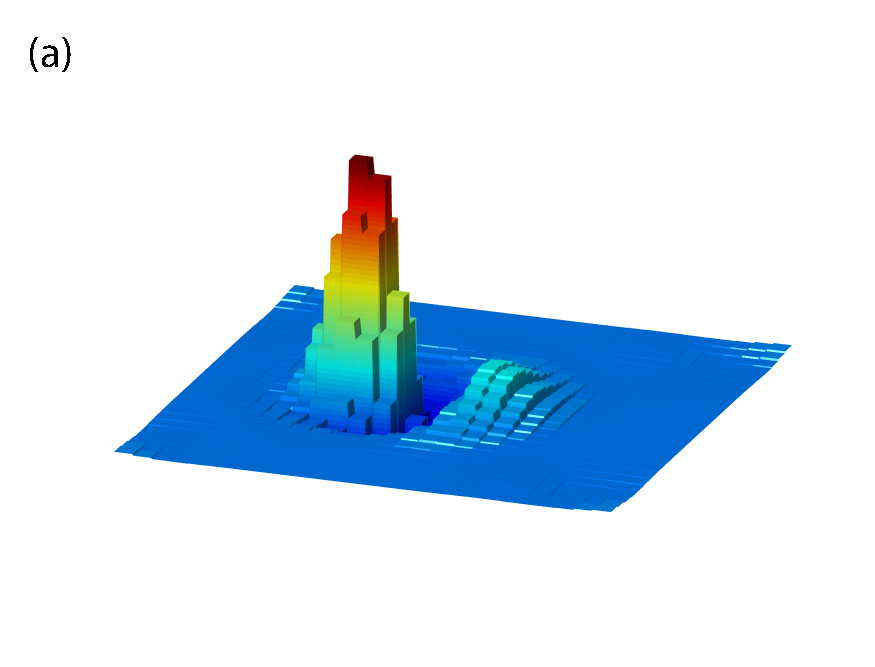
\includegraphics[height=.18\textheight]{images/27N_split_fourier.pdf}&
  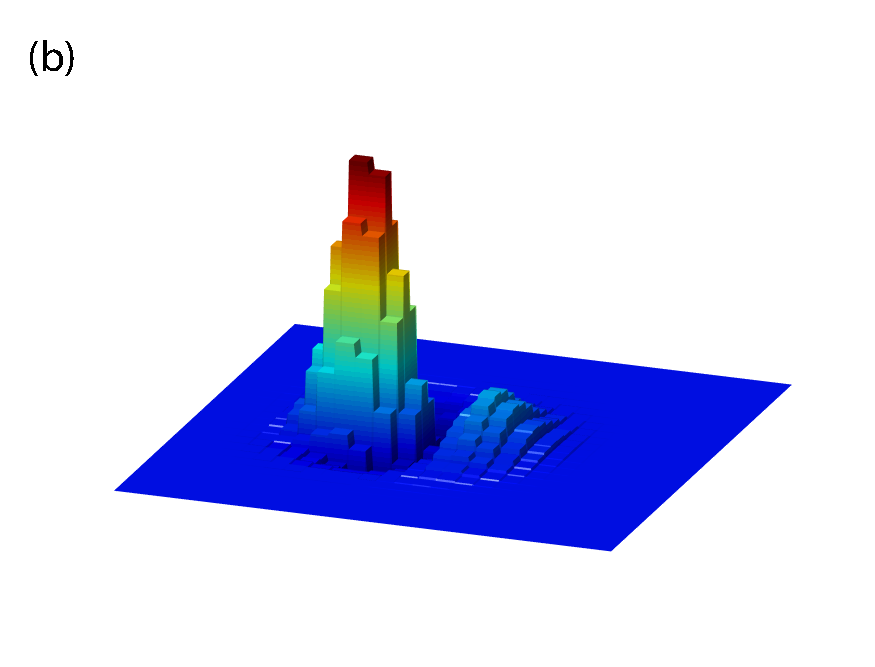
\includegraphics[height=.18\textheight]{images/27N_split_direct.pdf}&
  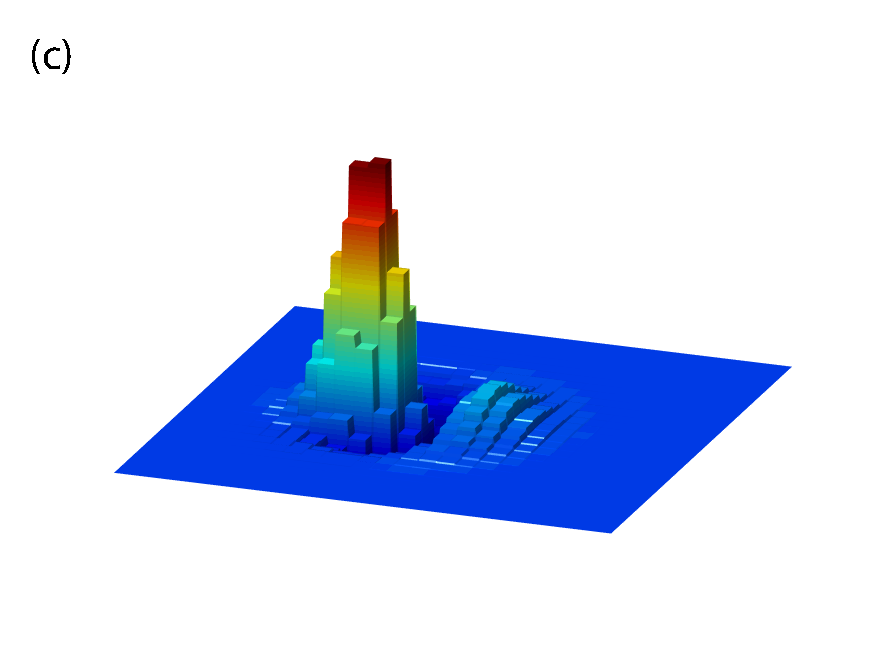
\includegraphics[height=.18\textheight]{images/27N_fourier.pdf}\\
  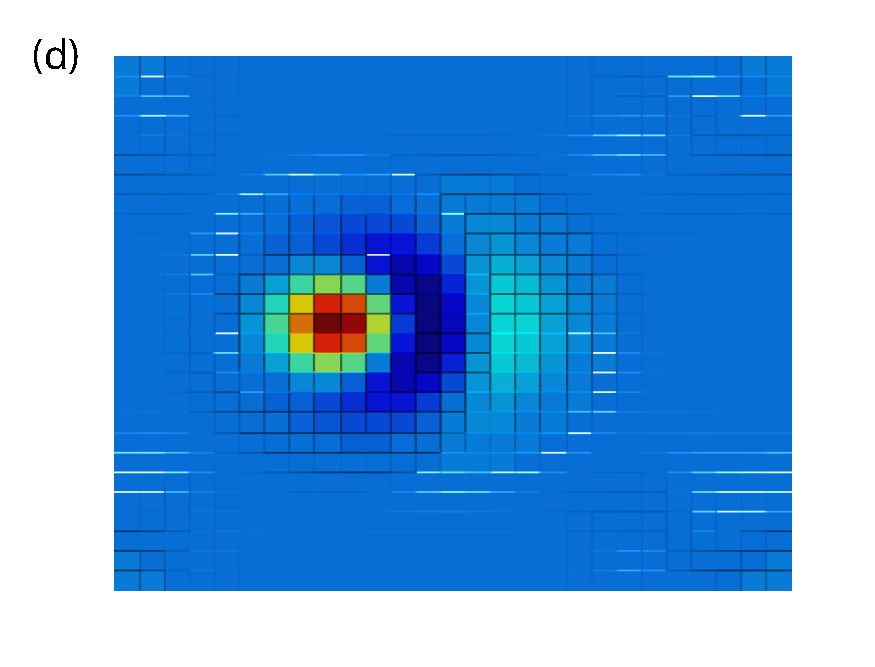
\includegraphics[height=.18\textheight]{images/27N_split_fourier_topdown.pdf}&
  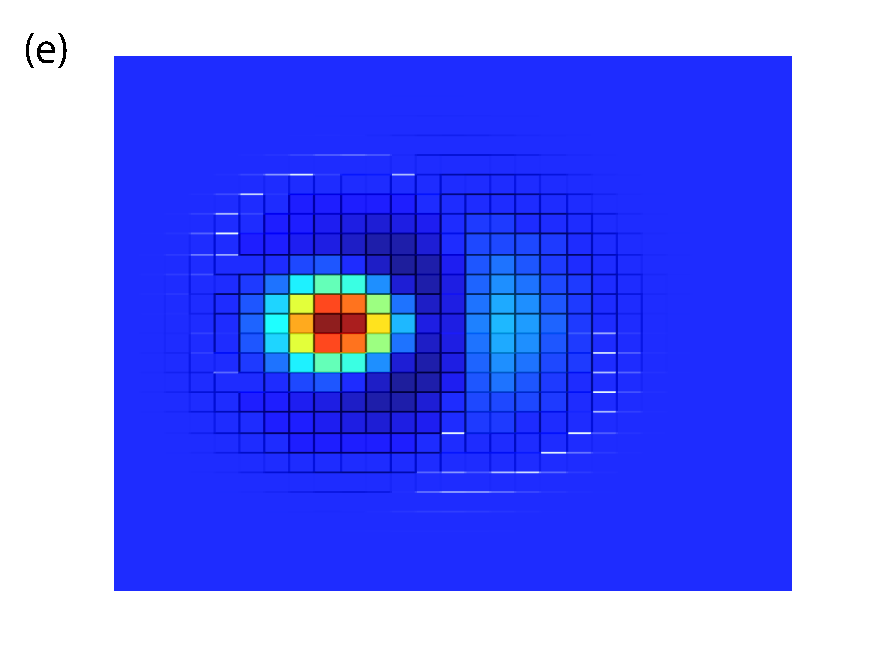
\includegraphics[height=.18\textheight]{images/27N_split_direct_topdown.pdf}&
  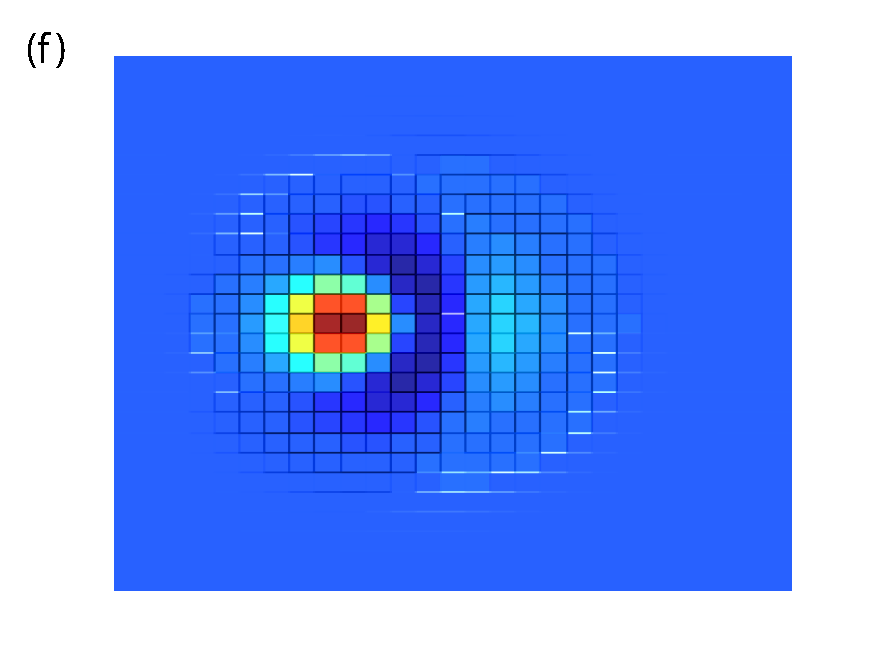
\includegraphics[height=.18\textheight]{images/27N_fourier_topdown.pdf}\\
\end{tabular}
\caption{\label{fig01} Evaluation of the collision operator using split and non-split forms: (a) and (d) the split form evaluated using the Fourier transform; (b) and (e) the split form evaluated directly; (c) and (f) the non-split form evaluated using the Fourier transform.}
\end{figure}
\end{center}

Another important issue that makes the non-split formulation more attractive is concerned 
with conservation of mass, momentum, and energy in the discrete solutions. It is the property of 
the exact Boltzmann collision operator that its mass, momentum, and temperature moments are zero. 
Generally, the conservation laws are satisfied only approximately when the Boltzmann equation is 
discretized. Many numerical approaches include mechanisms dedicated to enforcement of  
the conservation laws in discrete solutions in order to guarantee a physically meaningful result.

 \begin{table}[h]
  \begin{tabular}[c]{ c c c c c | c c c c }
  \hline
  \multicolumn{5}{c|}{Error in Conservation of Mass} &
  \multicolumn{4}{c}{Error in Conservation of Temperature}\\
    \hline 
    & \multicolumn{2}{c|}{Split} & \multicolumn{2}{c|}{Non-split} &
    \multicolumn{2}{c|}{Split} & \multicolumn{2}{c}{Non-split} \\
    \hline
    $n$ & Fourier& Direct & Fourier & Direct 
        & Fourier& Direct & Fourier & Direct \\
    \hline
    9   & 0.37 & 1.26 & 1.71E-5 & 1.92E-5 &
          3.51 & 1.69 & 1.71E-2 & 1.84E-2  \\
    15  & 0.10 & 1.20 & 1.45E-5 & 1.71E-5 & 
          0.29 & 1.25 & 1.64E-3 & 3.15E-3 \\
    21  & 0.18 & 1.18 & 0.67E-5 & 0.93E-5 & 
          1.38 & 1.24 & 5.61E-5 & 1.75E-3 \\
    27  & 0.18 & 1.18 & 0.61E-5 & 0.86E-5 & 
          1.37 & 1.24 & 5.40E-4 & 1.05E-3 \\
    \hline
  \end{tabular}
\caption{\label{tab02} Absolute errors in conservation of mass and temperature in the discrete collision integral computed using split and non-split formulations.}
\end{table}

It was observed that if no measures are introduced to enforce the conservation laws,  
solutions to the problem of spatially homogeneous relaxation obtained using the 
split formulation of the collision integral exhibit large, on the order of 5\%\ errors in 
temperature. The mass and momentum are also poorly conserved in this case. 
At the same time, solutions obtained using the non-split formulation had their mass, momentum,
and temperature accurate to three or more digits. To further explore this phenomena, 
we evaluated the collision operator in both split and non-split forms and computed its mass, 
momentum, and temperature moments. The solution was taken to be the sum of two Maxwellians 
in the example above. The numbers of velocity cells were 
varied from 9 to 27. In both split and non-split 
formulations of the collision integral, the decomposed form (\ref{dec01}) of the solution was 
used. For both forms, evaluation of the collision operator was done directly and using the Fourier transform. 
The results are summarized in Table~\ref{tab02}. It can be seen that errors in the mass and 
temperature in the non-split formulation are several orders of magnitude smaller than in 
the split formulation. The errors are also larger in the case of direct evaluation. 
A possible explanation to this is the combined effect of finite precision 
arithmetic and truncation errors in integration that lead to catastrophic cancellation 
when gain and loss terms are combined. 
We note that in 
both split and non-split forms, fulfilment of 
conservation laws requires exact cancellation of the respective integration 
sums. 
When the gain and
loss terms are computed separately using numerical quadratures, the 
relative truncation errors are expected to be acceptable for each of the terms. 
This may change, however, when the terms are combined. It is 
conceivable that significant digits cancel in the two terms and the 
truncation errors are promoted into significance, manifesting in strong 
violations of conservation laws. At the same time, increasing 
the number of velocity cells may not remedy the problem 
due to the expected accumulation of roundoff 
errors. Indeed, evaluation of the gain term in (\ref{eq:I_split}) requires 
$O(M^8)$ arithmetic operations. 
It is possible that combination of large and small values in the finite 
precision arithmetic results in loss of low order digits and a significant 
accumulation of roundoff. When the gain and loss terms are combined, 
this, again, will lead to loss of significance and to perturbations of 
conservation laws. In the case when both the  
non-split form and the decomposition (\ref{eq:I_decomp_continuous}) are used, 
much of the cancellation is happening 
on the level of the integrand. 
We hypothesize here 
that the resulting values of the integrand are smaller and vary less 
in scale. As a result, the accumulated absolute truncation and 
roundoff errors are also smaller, which gives better accuracy in 
conservation laws.

Because of the poor conservation properties and because of the 
susceptibility to aliasing errors we do not recommend the 
split form (\ref{eq:I_split}) for numerical implementation. 
\textbf{end copy and paste}

\section{0d Homogeneuous Relaxation COPY AND PASTED}

In this section we present results of solution of the problem of 
spatially homogeneous relaxation using Fourier evaluation of the 
collision operator. Two cases of initial data were considered. In 
both cases, the initial data is a sum of two Maxwellian densities. 
In the first case, the 
dimensionless densities, bulk velocities, and temperatures of the 
Maxwellians are $n_1=1.0007$, $n_2=2.9992$, 
$\bar{\vec{u}}_{1}=(1.2247,0,0)$, $\bar{\vec{u}}_{2}=(0.4082,0,0)$,
$T_{1}=0.2$, $T_{2}=0.7333$. These parameters correspond to upstream 
and downstream conditions of the Mach 3 normal shock wave.  
In the second case, we use the parameters of the example of the previous  
section: $n_{1}=1.6094$, $n_{2}=2.8628$, $\bar{\vec{u}}_{1}=(0.7750,0,0)$, $\bar{\vec{u}}_{2}=(0.4357,0,0)$, $T_{1}=0.3$, and $T_{2}=0.464$. These 
parameters correspond to upstream and downstream conditions of a Mach 1.55 
shock wave. 

In Figures~{\ref{fig02}} and {\ref{fig03}}, relaxation of moments in the 
Mach~3.0 and Mach~1.55 solutions are presented. In the case of Mach~3.0, 
$M=33$ velocity cells were used in each velocity dimension with one 
velocity node on each cell, $s=1$. In the case of Mach~1.55, $M=15$ and $s=1$ 
were used. In the computed solutions, the collision operator was evaluated 
both using the Fourier transform and directly. In the Mach 3.0 instance, the directional 
temperature moments were compared to the moments obtained from a DSMC solution
\cite{Boyd1991411}. 

\begin{center}
\begin{figure}[h]
\centering
  \begin{tabular}{@{}cc@{}}
  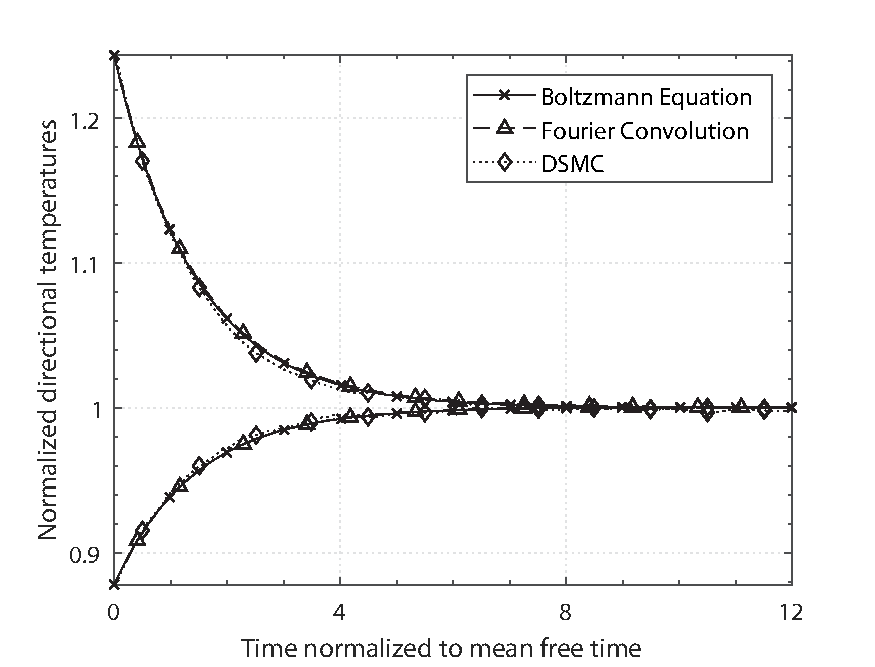
\includegraphics[height=.218\textheight]{images/m300_N33_mom2.pdf}&
  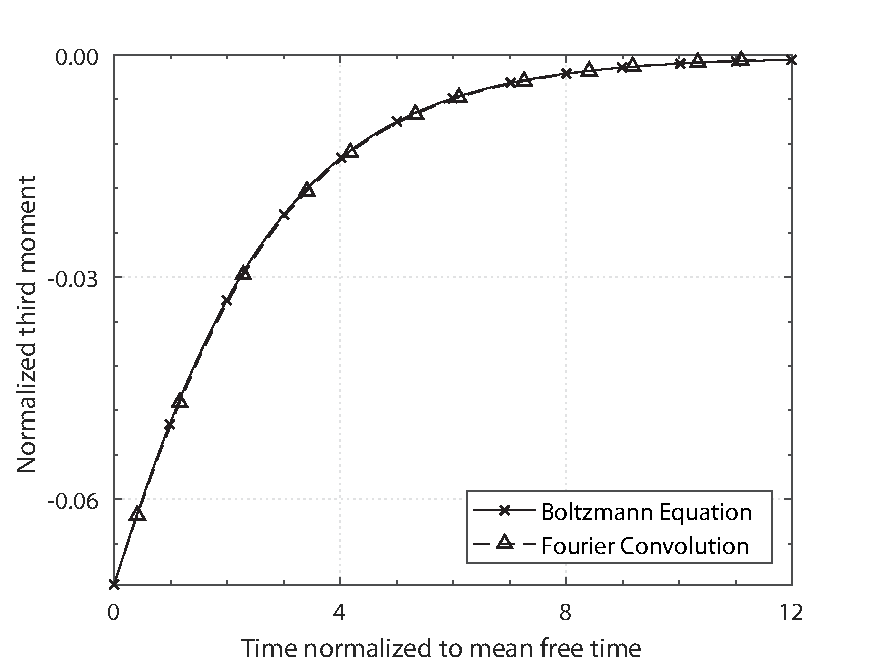
\includegraphics[height=.218\textheight]{images/m300_N33_mom3.pdf}\\      
  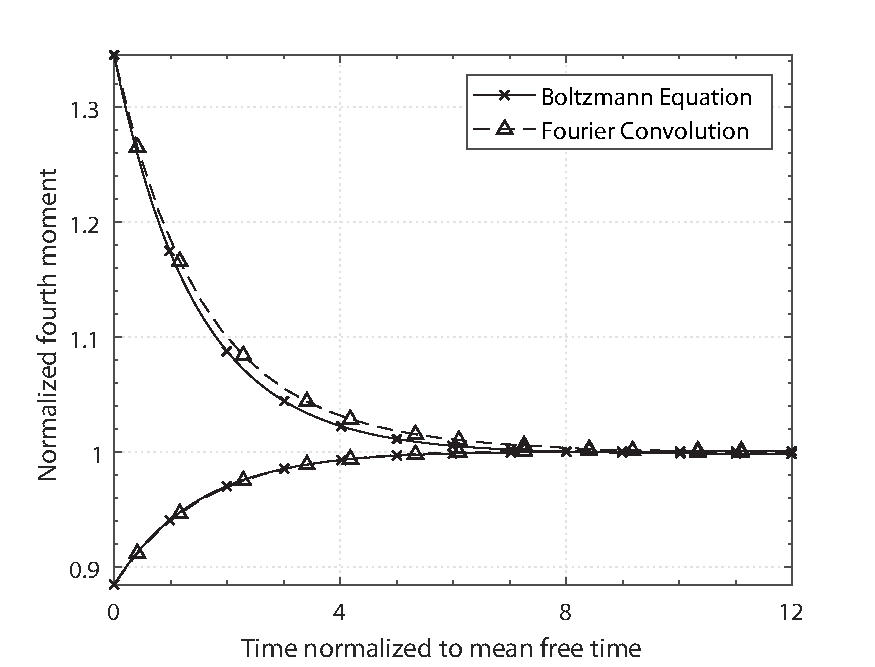
\includegraphics[height=.218\textheight]{images/m300_N33_mom4.pdf}&
  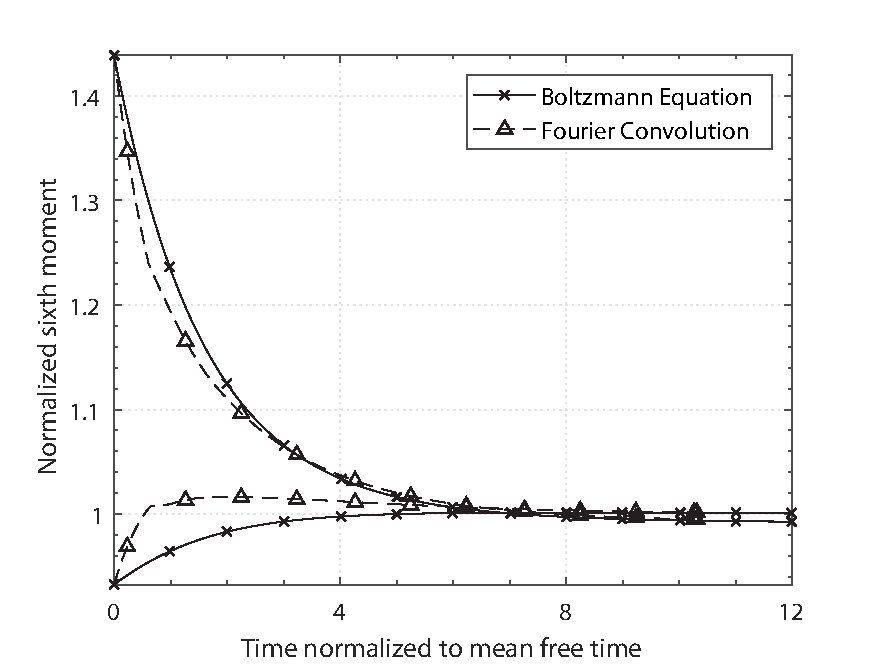
\includegraphics[height=.218\textheight]{images/m300_N33_mom6.pdf}\\
  \end{tabular}
\caption{\label{fig02} Relaxation of moments $f_{\varphi_{i,p}} = 
\int_{R^3} (u_{i}-\bar{u}_{i})^p f(t,\vec{u})\, du$, $i=1,2$, $p=2,3,4,6$ 
in a mix of Maxwellian streams corresponding to a shock wave with 
Mach number 3.0 obtained by solving the Boltzmann equation using Fourier and direct evaluations of the collision integral. In the case of $p=2$, the relaxation of moments 
is also compared to moments of a DSMC solution \cite{Boyd1991411}. }
\end{figure}
\end{center}

\begin{center}
\begin{figure}[h]
\centering
  \begin{tabular}{@{}cc@{}}
  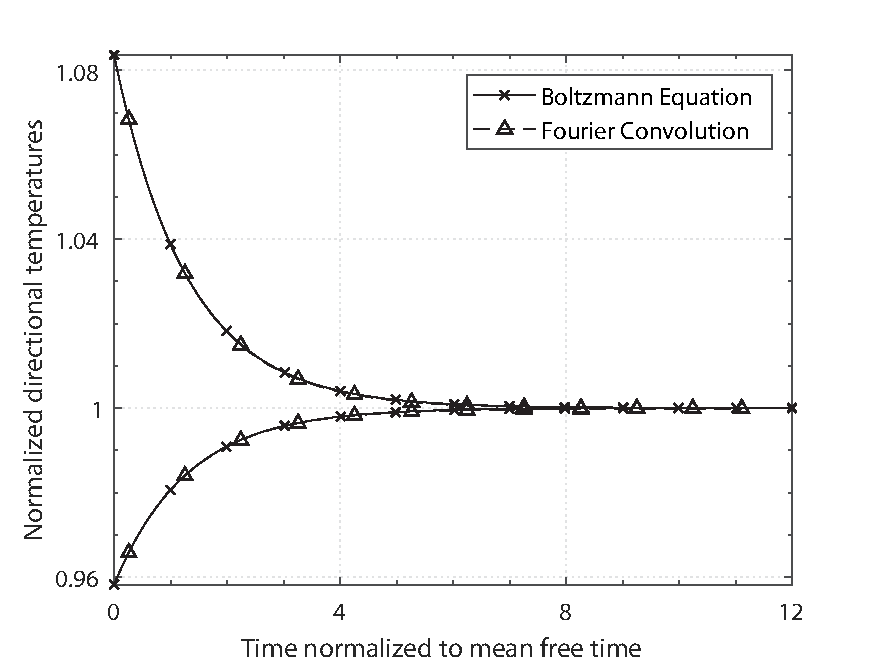
\includegraphics[height=.218\textheight]{images/m155_15N_mom2.pdf}&
  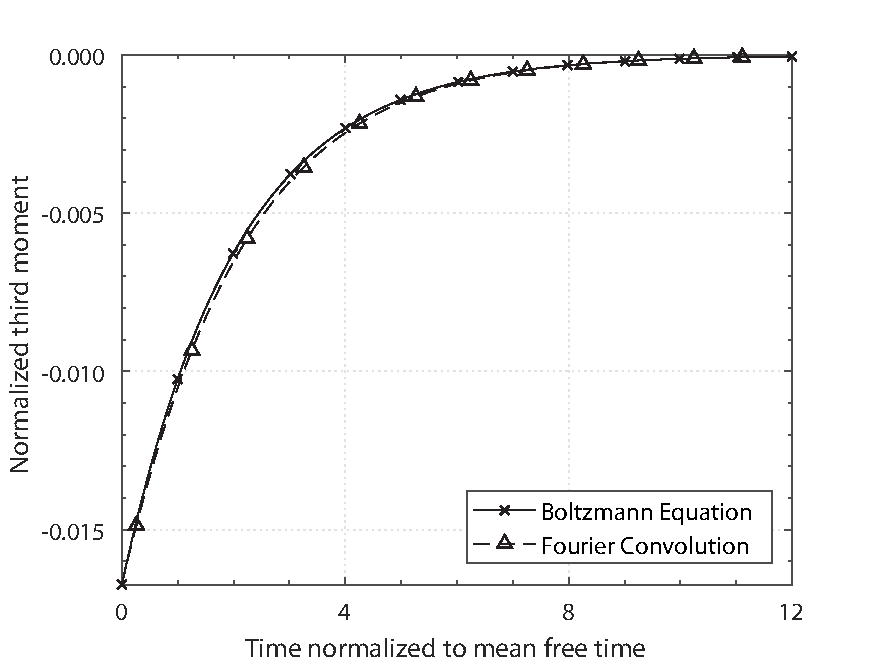
\includegraphics[height=.218\textheight]{images/m155_15N_mom3.pdf}\\      
  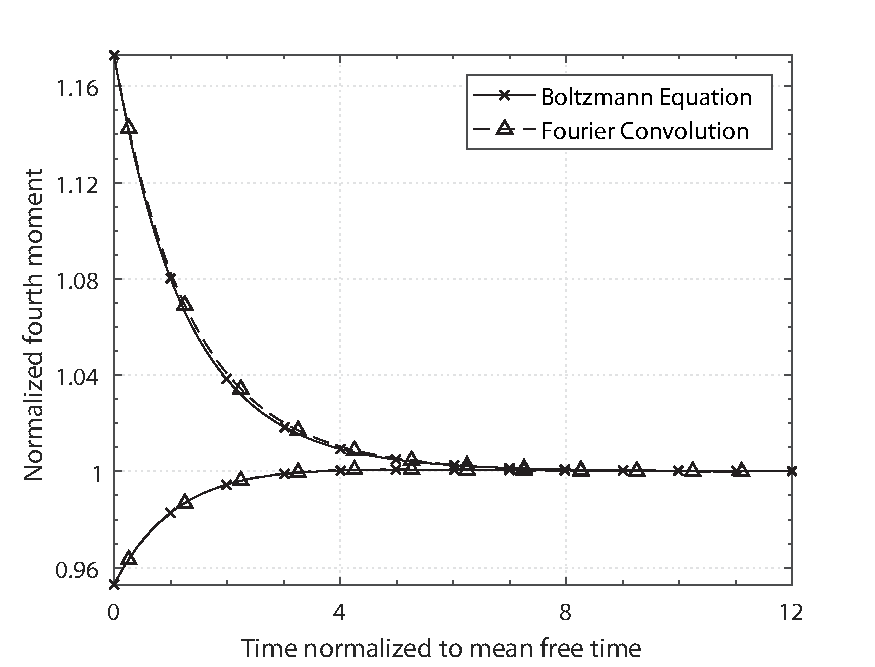
\includegraphics[height=.218\textheight]{images/m155_15N_mom4.pdf}&
  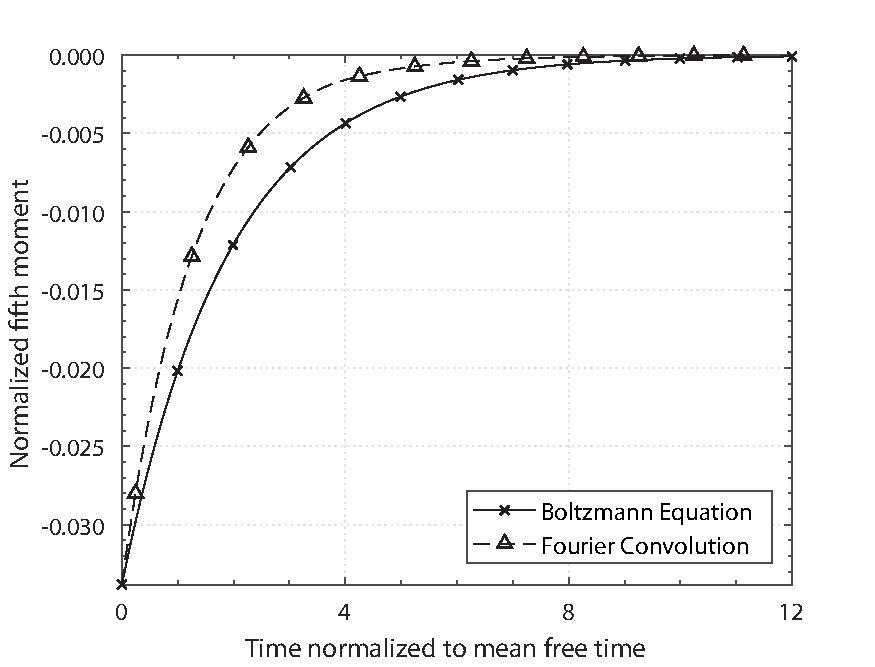
\includegraphics[height=.218\textheight]{images/m155_15N_mom6.pdf}\\
  \end{tabular}
\caption{\label{fig03} Relaxation of moments $f_{\varphi_{i,p}}$, $i=1,2$, $p=2,3,4,6$ 
in a mix of Maxwellian streams corresponding to a shock wave with 
Mach number 1.55 obtained by solving the Boltzmann equation using Fourier and direct evaluations of the collision integral.}
\end{figure}
\end{center}

It can be seen that the solutions obtained by the Fourier evaluation of the collision 
integral are close to those computed by the direct evaluation. The low order moments 
are in excellent agreement for both presented solutions. However, there are 
differences in the higher moments. It appears that the differences are caused 
by a small amount of the aliasing error in the solutions. This can be reduced 
by padding the solution and the kernel with zeros at the expense of higher numerical 
costs, both in time and memory. Overall, however, the $O(M^6)$ evaluation of 
the collision operator using the Fourier transform appears to be consistent 
and stable. 

\clearpage
\addcontentsline{toc}{chapter}{References}
\bibliographystyle{plain}
\bibliography{ffb10092017}
\end{document}